\documentclass[preprint,12pt]{elsarticle}

\usepackage{amsmath,amssymb,amsfonts,bm}
\usepackage{algorithmic}
\usepackage{algorithm}
\usepackage{array}
\usepackage{booktabs}
\usepackage{caption}
\usepackage{subcaption}
\usepackage{color}
\usepackage{float}
\usepackage{graphicx}
\usepackage{hyperref}
\usepackage{microtype}
\usepackage{multirow}
\usepackage{setspace}
\usepackage{textcomp}
\usepackage{url}
\usepackage{xcolor}

\setstretch{1.3}

\graphicspath{{results/figures/}{./}}

\hypersetup{
    colorlinks=true,
    linkcolor=blue,
    filecolor=magenta,
    citecolor=blue,
    urlcolor=blue
}
\usepackage{tikz}
\usetikzlibrary{arrows.meta,positioning,shapes.geometric,shapes.misc,fit,calc,decorations.pathreplacing}

\journal{Computerized Medical Imaging and Graphics / Artificial Intelligence in Medicine}

\begin{document}

\begin{frontmatter}

\title{Preoperative Clinical and OCT-Based Prediction of Visual Recovery After Macular Hole Surgery: An Uncertainty-Calibrated Multimodal Benchmark}

\author[inst1]{Sonali~Gupta\corref{cor1}}
\ead{sgupta_phd21@thapar.edu}

\cortext[cor1]{Corresponding author. Department of Computer Science and Engineering, Thapar Institute of Engineering and Technology, Patiala, Punjab 147004, India.}

\affiliation[inst1]{organization={Department of Computer Science and Engineering, Thapar Institute of Engineering and Technology},
            city={Patiala},
            postcode={147004},
            state={Punjab},
            country={India}}

\begin{highlights}
\item Multimodal prognostic benchmark evaluated under rigorous fold isolation across 25 Repeated Stratified CV folds and locked held-out test cohort ($n=17$).
\item Baseline visual acuity alone dominates binary visual outcome prediction ($\text{AUROC} = 82.70 \pm 8.31\%$), verified independent of chart ceiling effects ($p=0.0011$).
\item Resolves the multimodal fusion paradox in small samples ($n=104$): PCA-8 compression and regularized late fusion maximize continuous recovery variance ($R^2 = 0.485$, $\text{MAE} = 8.66$ letters).
\item First distribution-free cross-conformal prediction framework for macular hole prognosis, delivering $85.34\%$ empirical out-of-fold coverage with finite-sample guarantees.
\item Rigorous systematic comparison against verified prior benchmarks (Lachance 2021/2022, Obata 2021, Kucukgoz 2025 U-ARM evidential model).
\end{highlights}

\begin{abstract}
Idiopathic Full-Thickness Macular Hole (FTMH) surgery achieves anatomical closure in over 90\% of clinical cases, yet postoperative functional visual acuity (VA) recovery exhibits substantial, unexplained patient heterogeneity. Prior machine learning benchmarks on the standard CHU de Qu\'{e}bec cohort ($N=121$) were limited to arbitrary single train/test splits, evaluated only a coarse binary outcome threshold ($\ge 15$-letter gain on the ETDRS chart), provided uncalibrated point predictions, and experienced multimodal degradation when combining high-dimensional imaging representations with low-dimensional clinical tables. 

In this work, we present a fold-isolated, dual-task (binary classification and continuous regression) multimodal machine learning framework equipped with finite-sample, distribution-free uncertainty quantification. The benchmark cohort comprises 121 patients with seven preoperative clinical variables and dual-axis (horizontal and vertical cross-hair) High-Definition Optical Coherence Tomography (HD-OCT) B-scans. An auxiliary uncurated cohort of 373 records lacking standardized six-month follow-up was strictly excluded. Three preoperative feature tracks were engineered: (1) Preoperative clinical variables; (2) Classical geometric OCT morphometry (Minimum Linear Diameter [MLD], Basal Diameter, Hole Height, Macular Hole Index [MHI], and Tractional Hole Index [THI]); and (3) Siamese ImageNet-pretrained ResNet-50 deep embeddings compressed via fold-isolated Principal Component Analysis ($k=8$). Models were benchmarked using 25-fold Repeated Stratified Cross-Validation (5 repeats $\times$ 5 folds, $n=104$ development cohort) and evaluated once on a locked held-out test cohort ($n=17$).

Empirically, a single preoperative clinical variable—baseline visual acuity alone—achieved an AUROC of $82.70 \pm 8.31\%$ for binary classification, outperforming the full seven-variable clinical model ($80.70 \pm 9.97\%$) and published hybrid deep learning benchmarks ($81.9 \pm 5.2\%$). We confirm that this advantage is not an artifact of the ETDRS chart ceiling effect (non-ceiling subset: $+2.16\%$ advantage vs. $+2.00\%$ full cohort) and is consistent in direction across five independent cross-validation seeds (seed-level paired $t$-test, $t=8.426, p=0.0011$). In isolation, standalone OCT-derived features exhibited small-sample representation overfitting ($59.47 \pm 9.02\%$ AUROC in CV, collapsing to $34.7\%$ on the held-out test set). However, regularized multimodal late fusion of clinical features with deep vision embeddings yielded the top continuous visual recovery model ($R^2 = 0.485 \pm 0.137$, $\text{MAE} = 8.66 \pm 1.73$ letters). Out-of-fold cross-conformal prediction delivered well-calibrated distribution-free 90\% confidence intervals ($85.34 \pm 8.48\%$ empirical out-of-fold coverage at a radius of $\pm 14.05$ letters; test coverage $13/17 = 76.5\%$). This study establishes a transparent, reproducible benchmark and demonstrates the critical role of distribution-free uncertainty calibration for surgical decision support.
\end{abstract}

\begin{keywords}
Idiopathic Macular Hole \sep Optical Coherence Tomography (OCT) \sep Multimodal Deep Learning \sep Conformal Prediction \sep Uncertainty Quantification \sep Visual Acuity Regression \sep Vitreoretinal Surgery
\end{keywords}

\end{frontmatter}

% =========================================================================
\section{Introduction}
% =========================================================================

Idiopathic Full-Thickness Macular Hole (FTMH) is a primary cause of central vision loss in older adults, typically presenting in patients in their 60s and 70s with a well-documented female predominance ($\approx 70\%$)~\cite{kelly1991}. The condition occurs when incomplete posterior vitreous detachment exerts dynamic anteroposterior and tangential mechanical traction on the fovea, tearing through all neurosensory retinal layers from the internal limiting membrane (ILM) to the retinal pigment epithelium (RPE)~\cite{gass1995, duker2013, kusuhara2004}. As vitreous traction disrupts the delicate foveal architecture, patients experience progressive central vision loss, image distortion (metamorphopsia), and central blind spots~\cite{michalewska2010}. Without surgical intervention, prolonged exposure of the unroofed photoreceptors to intraocular fluid leads to irreversible cell death and permanent visual impairment~\cite{wakabayashi2010}.

Modern vitreoretinal surgery relies on pars plana vitrectomy (PPV) with ILM peeling and intraocular gas tamponade (e.g., sulfur hexafluoride [$\text{SF}_6$] or perfluoropropane [$\text{C}_3\text{F}_8$]), which achieves \textbf{anatomical hole closure in over 90\% to 95\% of cases}~\cite{kelly1991, brooks2000}. Yet this high anatomical success rate conceals a persistent clinical dilemma: \textbf{anatomical hole closure does not guarantee functional visual recovery}~\cite{baumann2021}. Among patients with identical anatomical outcomes, a subset achieves dramatic visual gains exceeding 3 to 4 lines on the Early Treatment Diabetic Retinopathy Study (ETDRS) chart ($\ge 15$ letters), while a substantial proportion shows minimal or no improvement, and some suffer permanent functional deficits from pre-existing photoreceptor loss or persistent microscopic synaptic disruption~\cite{wakabayashi2010, bottoni2011}. Accurate preoperative forecasting of this functional divergence is therefore central to patient counseling, setting realistic recovery expectations, and planning surgical timing.

\subsection{Related Work and Prior Prognostic Modeling}
The search for preoperative predictors of visual recovery has progressed through three distinct phases:

\subsubsection{Classical OCT Morphometry and Microstructural Integrity}
Clinicians initially turned to manual geometric calipers on cross-sectional OCT to forecast visual recovery. Ullrich et al.~\cite{ullrich2002} identified the Minimum Linear Diameter (MLD) as a primary prognostic marker, while Kusuhara et al.~\cite{kusuhara2004} introduced the Macular Hole Index ($\text{MHI} = \text{Hole Height} / \text{Basal Diameter}$), showing that taller, narrower holes with $\text{MHI} \ge 0.5$ generally achieve better postoperative vision. Subsequent indices, such as the Tractional Hole Index ($\text{THI} = \text{Height} / \text{MLD}$)~\cite{ruizmoreno2008} and Diameter Hole Index ($\text{DHI}$), built on the same geometric premise.

Yet these measurements describe only the macro-architecture of the defect, overlooking the biological health of the surrounding neural tissue. Microstructural studies by Wakabayashi et al.~\cite{wakabayashi2010}, Bottoni et al.~\cite{bottoni2011}, Shimozono et al.~\cite{shimozono2011}, and Baumann et al.~\cite{baumann2021} later revealed that postoperative visual recovery actually hinges on outer retinal restoration—specifically whether the External Limiting Membrane (ELM) and Ellipsoid Zone (EZ) reconstitute following surgery. However, reliably segmenting and quantifying these delicate microscopic layers on OCT is notoriously difficult, even with automated segmentation architectures such as U-Net~\cite{ronneberger2015} and deep graph-search formulations~\cite{fang2017}. This challenge led Singh et al.~\cite{singh2022} to curate a dedicated 5,243-slice public benchmark across 107 patients, highlighting both the clinical value and the technical complexity of automated ELM boundary detection.

\subsubsection{Deep Learning on Clinical and OCT Data}
Following foundational breakthroughs in clinical deep learning for retinal disease diagnosis and referral~\cite{defauw2018}, machine learning emerged as a way to extract predictive representations without relying on manual caliper measurements. Lachance et al.~\cite{lachance2021} first explored this on the standardized, publicly released CHU de Qu\'{e}bec cohort ($N=121$), reporting $75.0\%$ AUROC from seven preoperative clinical features and $72.8 \pm 14.6\%$ from a convolutional neural network (\texttt{CBR-Tiny}) trained directly on preoperative OCT B-scans for binary visual gain ($\ge 15$ letters). In a follow-up study, Lachance et al.~\cite{lachance2022} refined the clinical baseline to $80.6 \pm 7.2\%$ AUROC and combined it with the OCT-based CNN in a late-fusion hybrid model, reaching $81.9 \pm 5.2\%$. Their central finding—that combining OCT-derived representations with clinical features yielded only a modest, non-significant gain over clinical variables alone—has since served as a cautionary benchmark for small-sample multimodal ophthalmic AI.

\subsubsection{Continuous Acuity Regression and Uncertainty Quantification}
Parallel efforts have moved toward continuous visual acuity prediction and individual-level uncertainty quantification. Obata et al.~\cite{obata2021} developed a deep learning approach predicting four-class ordinal visual acuity tiers ($R^2 = 0.52$, $p < 0.005$). Kucukgoz et al.~\cite{kucukgoz2024} utilized dense 3D OCT volumes (49 scans per eye, $N=210$) across nine deep architectures to predict continuous postoperative acuity, achieving $\text{MAE} = 6.47$ letters ($R^2 = 0.52$). Most recently, Kucukgoz et al.~\cite{kucukgoz2025} introduced the Uncertainty-Aware Retinal Model (U-ARM), employing deep evidential regression with a parametric Normal-Inverse-Gamma (NIG) prior. Notably, U-ARM was evaluated directly on the same public CHU de Qu\'{e}bec dataset used here, reporting an internal test $\text{MAE} = 6.49 \pm 0.26$ letters ($R^2 = 0.42, p < 0.005$) and an external test $\text{MAE} = 6.97 \pm 0.28$ letters ($R^2 = 0.40, p = 0.039$) for three-month visual acuity.

\begin{table*}[!t]
\centering
\caption{Systematic Benchmark Comparison of Prior Literature and Proposed Multimodal Conformal Framework}
\label{tab:sota_comparison}
\resizebox{\textwidth}{!}{%
\begin{tabular}{lcccccc}
\toprule
\textbf{Study / Reference} & \textbf{Year} & \textbf{Cohort Dataset} & \textbf{Sample Size ($N$)} & \textbf{Prognostic Task \& Endpoint} & \textbf{Best Reported Result} & \textbf{Uncertainty Quantification} \\
\midrule
Lachance \textit{et al.}~\cite{lachance2021} & 2021 & HD-OCT of MH & 121 & Binary Gain ($\ge 15$ letters) & $\text{AUROC} = 75.0\%$ (CNN: $72.8\%$) & None \\
Lachance \textit{et al.}~\cite{lachance2022} & 2022 & HD-OCT of MH & 121 & Binary Gain ($\ge 15$ letters) & $\text{AUROC} = 81.9\%$ (Clinical: $80.6\%$) & None \\
Obata \textit{et al.}~\cite{obata2021} & 2021 & Clinical Cohort & --- & 4-Tier Ordinal Staging & $R^2 = 0.52, \; p < 0.005$ & None \\
Kucukgoz \textit{et al.}~\cite{kucukgoz2024} & 2024 & OCT-Newcastle 3D & 210 & Continuous Postop VA & $\text{MAE} = 6.47, \; R^2 = 0.52$ & None \\
Kucukgoz \textit{et al.} (U-ARM, Internal)~\cite{kucukgoz2025} & 2025 & HD-OCT of MH & 320 imgs & Continuous 3-Month VA & $\text{MAE} = 6.49, \; R^2 = 0.42$ & Evidential (Parametric NIG) \\
Kucukgoz \textit{et al.} (U-ARM, External)~\cite{kucukgoz2025} & 2025 & HD-OCT of MH & --- & Continuous 3-Month VA & $\text{MAE} = 6.97, \; R^2 = 0.40$ & Evidential (Parametric NIG) \\
\midrule
\textbf{This Work (Proposed)} & \textbf{2026} & \textbf{HD-OCT of MH} & \textbf{121 (104 Dev / 17 Test)} & \textbf{Dual: Continuous 6mo $\Delta\text{VA}$ + Binary} & $\mathbf{R^2 = 0.485\text{--}0.557, \; \text{AUROC} = 82.7\%}$ & \textbf{Conformal (Distribution-Free)~\cite{vovk2005, angelopoulos2021}} \\
\bottomrule
\end{tabular}}
\end{table*}

\subsection{Open Clinical and Methodological Gaps}
As summarized in Table~\ref{tab:sota_comparison}, existing prognostic literature leaves three core challenges unaddressed:
\begin{enumerate}
    \item \textbf{Arbitrary Binary Outcome Thresholds and Chart Ceilings:} Framing prognosis strictly as a binary threshold ($\ge 15$-letter gain) discards recovery granularity. Patients presenting with good baseline vision ($>65$ letters) cannot gain 15 letters due to the 100-letter ETDRS chart ceiling, penalizing models for patients who achieve excellent surgical outcomes. Furthermore, prior binary studies evaluated only a single arbitrary train/test split without testing if findings survive repeated resampling or formal variance-corrected significance testing~\cite{nadeau2003}.
    \item \textbf{The Multimodal Small-Sample Paradox:} Combining high-dimensional deep vision embeddings ($2048$-D) with tabular clinical data in small medical cohorts ($N \approx 100$) introduces severe feature noise, which often degrades the performance of strong clinical baselines unless regularized with fold-isolated dimensionality reduction.
    \item \textbf{Rigid Parametric Uncertainty Assumptions:} Prior uncertainty estimation in retinal surgery relies on parametric evidential distributions (e.g., Normal-Inverse-Gamma priors). These assume residual normality, which may fail in small, heterogeneous clinical cohorts. A distribution-free, finite-sample uncertainty calibration grounded in conformal prediction theory~\cite{vovk2005, angelopoulos2021} has not been previously established for macular hole surgery.
\end{enumerate}

\subsection{Key Contributions}
To resolve these challenges, this study establishes a leak-free, dual-task multimodal framework evaluated under 25-fold Repeated Stratified Cross-Validation and an independent locked test set:
\begin{itemize}
    \item \textbf{Dual-Task Prognostic Architecture:} We model both binary functional gain ($\ge 15$ letters) and continuous visual recovery ($\Delta \text{VA} = \text{VA}_{6\text{mo}} - \text{VA}_{\text{baseline}}$), capturing granular surgical trajectories across the full visual spectrum.
    \item \textbf{Dominance and Robustness of Preoperative Acuity:} We demonstrate that baseline visual acuity alone achieves $82.70 \pm 8.31\%$ AUROC for binary classification, confirm that this advantage is not driven by chart ceiling effects, and verify its consistency across multiple random seeds ($p=0.0011$).
    \item \textbf{Distribution-Free Conformal Prediction:} Grounded in the conformal prediction framework of Vovk et al.~\cite{vovk2005} and Angelopoulos and Bates~\cite{angelopoulos2021}, we introduce the first out-of-fold cross-conformal prediction framework for macular hole prognosis, delivering $85.34 \pm 8.48\%$ empirical coverage at a calibrated radius of $\pm 14.05$ letters without parametric distribution assumptions.
    \item \textbf{Transparent Negative Findings on Standalone Deep Embeddings:} We document the representation overfitting of uncompressed deep vision embeddings in small cohorts ($59.47\%$ in CV to $34.7\%$ on test), providing key methodological insights for multimodal ophthalmic AI.
\end{itemize}

% =========================================================================
\section{Proposed Methodology and Multimodal Framework}
\label{sec:methodology}
% =========================================================================

\subsection{Mathematical Notations and Formal Problem Formulation}
\label{sec:notations_problem_formulation}

To establish a mathematically rigorous foundation for all multimodal representations, prognostic predictions, and uncertainty guarantees, we define the complete formal notations, operational spaces, and governing equations employed throughout this framework.

\noindent\textbf{Observation Spaces and Multimodal Tuples:} Let $\mathcal{D} = \{ \mathbf{z}_i \}_{i=1}^N$ denote the benchmark dataset of $N=121$ patient records drawn exchangeably from an underlying distribution $\mathcal{P}_{\mathcal{Z}}$. Each individual patient observation is represented by a multimodal tuple:
\begin{equation}
\mathbf{z}_i = \left( \mathbf{c}_i^{\text{raw}},\, \mathbf{I}_{i,H},\, \mathbf{I}_{i,V},\, y_i^{\text{post}} \right) \in \mathcal{Z},
\end{equation}
where $\mathbf{c}_i^{\text{raw}} = [c_{i,1}^{\text{raw}}, \dots, c_{i,7}^{\text{raw}}]^{\top} \in \mathbb{R}^7$ denotes the raw preoperative vector of seven clinical and demographic variables (\texttt{age}, \texttt{sex}, \texttt{pseudophakic}, \texttt{mh\_duration}, \texttt{elevated\_edge}, \texttt{mh\_size}, and \texttt{va\_baseline}); $\mathbf{I}_{i,H}, \mathbf{I}_{i,V} \in \mathbb{R}^{496 \times 768}$ denote the raw high-resolution horizontal and vertical foveal cross-hair Optical Coherence Tomography (HD-OCT) B-scans; and $y_i^{\text{post}} = \text{VA}_i^{6\text{mo}} \in \mathbb{R}$ represents the ground-truth post-operative Best-Corrected Visual Acuity measured at the standardized six-month surgical follow-up on the ETDRS letter chart.

\noindent\textbf{Dual-Task Learning Objectives:} Post-operative visual recovery is formulated as a dual-task learning problem providing both clinical risk stratification and continuous functional recovery tracking:
\begin{enumerate}
    \item \textbf{Primary Task (Binary Surgical Gain):} Predict whether an eye achieves substantial functional visual recovery ($\ge 3$ ETDRS lines, or $15$ letters) at six months post-vitrectomy:
    \begin{equation}
    y_i^{\text{bin}} = \mathbb{I}\left(\text{VA}_i^{6\text{mo}} - \text{VA}_i^{\text{baseline}} \ge 15 \text{ ETDRS letters}\right) \in \{0, 1\},
    \end{equation}
    where $\mathbb{I}(\cdot)$ is the indicator function evaluating to $1$ for substantial visual recovery and $0$ otherwise.
    \item \textbf{Secondary Task (Continuous Recovery Regression):} Predict the net continuous change in visual acuity:
    \begin{equation}
    y_i^{\text{reg}} = \Delta \text{VA}_i = \text{VA}_i^{6\text{mo}} - \text{VA}_i^{\text{baseline}} \in \mathbb{R}.
    \end{equation}
\end{enumerate}

\noindent\textbf{In-Fold Clinical Preprocessing and Scaling:} For each patient $i$, raw clinical vectors $\mathbf{c}_i^{\text{raw}}$ are sanitized by converting sentinel $-9$ values into explicit nulls, followed by in-fold median imputation. To prevent optimistic evaluation bias across cross-validation folds, $z$-score standardization parameters are calculated strictly from training partition instances $\mathcal{D}_{\text{train}}$:
\begin{equation}
\mu_j = \frac{1}{|\mathcal{D}_{\text{train}}|} \sum_{i \in \mathcal{D}_{\text{train}}} c_{i,j}^{\text{imputed}}, \quad \sigma_j = \sqrt{\frac{1}{|\mathcal{D}_{\text{train}}| - 1} \sum_{i \in \mathcal{D}_{\text{train}}} \left( c_{i,j}^{\text{imputed}} - \mu_j \right)^2},
\end{equation}
yielding the standardized in-fold clinical feature vector:
\begin{equation}
\mathbf{x}_i^{\text{clin}} = \left( \mathbf{c}_i^{\text{imputed}} - \bm{\mu}_{\text{train}} \right) \oslash \left( \bm{\sigma}_{\text{train}} + \epsilon \right) = \left[ \frac{c_{i,1}^{\text{imputed}} - \mu_1}{\sigma_1 + \epsilon}, \; \dots, \; \frac{c_{i,7}^{\text{imputed}} - \mu_7}{\sigma_7 + \epsilon} \right]^{\top} \in \mathbb{R}^7,
\end{equation}
where $\oslash$ denotes element-wise Hadamard division and $\epsilon = 10^{-8}$ is a numerical stabilizer.

\noindent\textbf{OCT Standardization and Siamese Vision Embeddings:} Raw dual-axis B-scans $(\mathbf{I}_{i,H}, \mathbf{I}_{i,V})$ undergo min-max intensity normalization and fovea-aligned center cropping to $\mathbb{R}^{448 \times 448}$:
\begin{equation}
\tilde{I}(x, y) = \frac{I(x, y) - \min(I)}{\max(I) - \min(I) + 10^{-6}}.
\end{equation}
Let $\phi: \mathbb{R}^{448 \times 448} \to \mathbb{R}^{2048}$ denote an ImageNet-pretrained ResNet-50 feature extractor truncated prior to the final classification head. Foveal representations from horizontal and vertical cross-hairs are fused via symmetric dual-meridian mean pooling:
\begin{equation}
\mathbf{f}_i = \frac{1}{2}\left( \phi(\tilde{\mathbf{I}}_{i,H}) + \phi(\tilde{\mathbf{I}}_{i,V}) \right) \in \mathbb{R}^{2048}.
\end{equation}

\noindent\textbf{Fold-Isolated Dimensionality Reduction (PCA-8):} To prevent small-sample representation overfitting ($N \approx 100$), Principal Component Analysis (PCA) is fitted on training-fold deep embeddings $\{\mathbf{f}_j\}_{j \in \mathcal{D}_{\text{train}}}$. The empirical sample covariance matrix $\mathbf{\Sigma}_f \in \mathbb{S}_{+}^{2048}$ is computed via:
\begin{equation}
\mathbf{\Sigma}_f = \frac{1}{|\mathcal{D}_{\text{train}}| - 1} \sum_{i \in \mathcal{D}_{\text{train}}} (\mathbf{f}_i - \bm{\mu}_f)(\mathbf{f}_i - \bm{\mu}_f)^{\top}.
\end{equation}
Spectral decomposition $\mathbf{\Sigma}_f \mathbf{v}_m = \lambda_m \mathbf{v}_m$ yields the top $k=8$ orthogonal eigenvectors $\mathbf{V}_k = [\mathbf{v}_1, \dots, \mathbf{v}_8] \in \mathbb{R}^{2048 \times 8}$, projecting high-dimensional vision latents into an 8-dimensional compressed subspace:
\begin{equation}
\mathbf{x}_i^{\text{vis}} = \mathbf{V}_k^{\top} \left( \mathbf{f}_i - \bm{\mu}_f \right) \in \mathbb{R}^8.
\end{equation}

\noindent\textbf{Automated Macro-Morphometry Features:} From calibrated foveal calipers of Minimum Linear Diameter ($\text{MLD}_i$), Basal Diameter ($\text{BD}_i$), and Hole Height ($H_i$), three scale-invariant geometric ratios are derived:
\begin{equation}
\text{MHI}_i = \frac{H_i}{\text{BD}_i}, \quad \text{THI}_i = \frac{H_i}{\text{MLD}_i}, \quad \text{DHI}_i = \frac{\text{BD}_i - \text{MLD}_i}{H_i},
\end{equation}
yielding the 6-dimensional morphometric descriptor $\mathbf{x}_i^{\text{morph}} = [\text{MLD}_i, \text{BD}_i, H_i, \text{MHI}_i, \text{THI}_i, \text{DHI}_i]^{\top} \in \mathbb{R}^6$.

\noindent\textbf{Multimodal Feature Concatenation and Supervised Optimization:} Multimodal integration concatenates clinical priors with compressed deep vision embeddings:
\begin{equation}
\mathbf{x}_i^{\text{multimodal}} = \left[ (\mathbf{x}_i^{\text{clin}})^{\top},\; (\mathbf{x}_i^{\text{vis}})^{\top} \right]^{\top} \in \mathbb{R}^{15}.
\end{equation}
Model parameters for continuous regression are optimized across training instances via:
\begin{align}
\hat{\mathbf{w}}_{\text{ridge}} &= \arg\min_{\mathbf{w}} \sum_{i \in \mathcal{D}_{\text{train}}} \left( y_i^{\text{reg}} - \mathbf{w}^{\top}\mathbf{x}_i^{\text{multimodal}} \right)^2 + \lambda \|\mathbf{w}\|_2^2, \\
\hat{g}_{\text{GBDT}} &= \arg\min_{g \in \mathcal{H}_{\text{tree}}} \sum_{i \in \mathcal{D}_{\text{train}}} \mathcal{L}_{\text{Huber}}\left( y_i^{\text{reg}},\, g(\mathbf{x}_i^{\text{multimodal}}) \right) + \Omega(g),
\end{align}
where $\lambda = 1.0$ is the $L_2$ regularization coefficient, $\Omega(g)$ penalizes tree complexity, and the robust Huber loss with threshold $\delta = 1.35$ is defined as:
\begin{equation}
\mathcal{L}_{\text{Huber}}(y, \hat{y}) = \begin{cases} 
\frac{1}{2}(y - \hat{y})^2, & \text{if } |y - \hat{y}| \le \delta, \\
\delta |y - \hat{y}| - \frac{1}{2}\delta^2, & \text{otherwise}.
\end{cases}
\end{equation}

\noindent\textbf{Ensemble Prediction and Binary Classification Mapping:} Continuous visual acuity predictions are synthesized via an equally weighted late-fusion ensemble:
\begin{equation}
\hat{\mu}(\mathbf{x}_i) = \frac{1}{2}\hat{\mathbf{w}}_{\text{ridge}}^{\top}\mathbf{x}_i^{\text{multimodal}} + \frac{1}{2}\hat{g}_{\text{GBDT}}(\mathbf{x}_i^{\text{multimodal}}) \in \mathbb{R}.
\end{equation}
For binary surgical success classification, calibrated posterior class probabilities are computed via:
\begin{equation}
\hat{p}_i = \sigma\left( \hat{\mathbf{w}}_{\text{clf}}^{\top}\mathbf{x}_i \right) = \frac{1}{1 + \exp\left(-\hat{\mathbf{w}}_{\text{clf}}^{\top}\mathbf{x}_i\right)} \in [0, 1].
\end{equation}

\noindent\textbf{Distribution-Free Out-of-Fold Cross-Conformal Uncertainty Calibration:} To equip point forecasts with rigorous patient-specific confidence bounds without parametric normality assumptions, let $s_i \in \mathbb{R}_{\ge 0}$ denote the absolute residual non-conformity score evaluated on out-of-fold validation instances:
\begin{equation}
s_i = |y_i - \hat{\mu}(\mathbf{x}_i)|.
\end{equation}
For a user-specified significance level $\alpha \in (0, 1)$ (target coverage $1-\alpha = 0.90$), the calibrated conformal quantile threshold $\hat{q} \in \mathbb{R}_{>0}$ is computed at index $p = \frac{\lceil (n_{\text{dev}}+1)(1-\alpha) \rceil}{n_{\text{dev}}}$:
\begin{equation}
\hat{q} = \text{Quantile}\left( \{s_i\}_{i=1}^{n_{\text{dev}}}, \; \min(1.0, p) \right).
\end{equation}
For any unseen test patient $\mathbf{x}_{n+1}$, the distribution-free prediction interval:
\begin{equation}
\mathcal{C}_{1-\alpha}(\mathbf{x}_{n+1}) = \left[ \hat{\mu}(\mathbf{x}_{n+1}) - \hat{q}, \;\; \hat{\mu}(\mathbf{x}_{n+1}) + \hat{q} \right] \subset \mathbb{R}
\end{equation}
satisfies the exact finite-sample marginal coverage guarantee:
\begin{equation}
\mathbb{P}\left( y_{n+1} \in \mathcal{C}_{1-\alpha}(\mathbf{x}_{n+1}) \right) \ge 1 - \alpha.
\end{equation}

\noindent\textbf{Resampled Significance Testing (Nadeau--Bengio Correction):} In repeated cross-validation ($J = K \times R = 25$ total evaluation folds), standard paired $t$-tests underestimate variance due to overlapping training sets. Let $d_j \in \mathbb{R}$ denote the performance metric difference between two models on fold $j \in \{1, \dots, J\}$, and let $\bar{d} = \frac{1}{J}\sum_{j=1}^J d_j$ denote the mean difference across folds. The sample variance across folds is:
\begin{equation}
S_d^2 = \frac{1}{J-1} \sum_{j=1}^J \left( d_j - \bar{d} \right)^2.
\end{equation}
The Nadeau--Bengio corrected test statistic $t_{\text{NB}}$ is defined as:
\begin{equation}
t_{\text{NB}} = \frac{\bar{d}}{\sqrt{\left( \frac{1}{J} + \frac{n_{\text{val}}}{n_{\text{train}}} \right) S_d^2}},
\end{equation}
where $n_{\text{val}} = 21$ and $n_{\text{train}} = 83$, which is compared against Student's $t$-distribution with $J-1 = 24$ degrees of freedom.

\subsection{Dataset Description and Cohort Partitioning}
\label{sec:dataset_partitioning}
This study utilizes the publicly available High-Definition Optical Coherence Tomography (HD-OCT) Macular Hole Dataset originating from the Centre Hospitalier Universitaire (CHU) de Qu\'{e}bec (collected between 2014 and 2018 by Dr. Mathieu Godbout and colleagues)~\cite{lachance2021, lachance2022}. The public repository contains 494 total patient records organized across four partitions: \texttt{train} ($n=83$), \texttt{val} ($n=21$), \texttt{test} ($n=17$), and an uncurated auxiliary partition \texttt{others} ($n=373$).

To prevent optimistic evaluation bias, strict cohort auditing was applied:
\begin{enumerate}
    \item \textbf{Benchmark Cohort ($N=121$):} Consists of the 121 consecutive patients with complete preoperative clinical data, two high-resolution cross-hair OCT B-scans (horizontal and vertical foveal meridians), and standardized 6-month postoperative ETDRS visual acuity follow-up, directly matching the cohort evaluated by Lachance et al.~\cite{lachance2021, lachance2022}.
    \begin{itemize}
        \item \textbf{Development Cohort ($n=104$):} Formed by merging the original \texttt{train} ($83$) and \texttt{val} ($21$) subsets. All model training, cross-validation ablation, hyperparameter tuning, and conformal quantile calibration were performed strictly within this partition using 25-fold Repeated Stratified CV.
        \item \textbf{Locked Held-Out Test Cohort ($n=17$):} Corresponds to the standard locked \texttt{test} partition (Patient IDs 104--120; 8 positive cases [$\ge 15$ letters], 9 negative cases). This set was evaluated exactly once after all modeling decisions were permanently frozen.
    \end{itemize}
    \item \textbf{Auxiliary Cohort ($n=373$):} Records in \texttt{others} lacked standardized six-month visual acuity measurements and complete tabular records and were completely excluded from all supervised training, feature selection, and evaluation protocols.
\end{enumerate}

The partition structure of the dataset is summarised in Table~\ref{tab:dataset_partitions}.

\begin{table}[t]
\centering
\caption{Dataset partition structure and benchmark protocol allocation.}
\label{tab:dataset_partitions}
\renewcommand{\arraystretch}{1.1}
\footnotesize
\begin{tabular}{lcl}
\toprule
\textbf{Partition} & \textbf{Sample Size ($n$)} & \textbf{Role in Benchmark Protocol} \\
\midrule
Development (\texttt{train} + \texttt{val}) & 104 & 25-Fold Repeated Stratified CV, Hyperparameter Tuning \\
Locked Test (\texttt{test}) & 17 & Single-Pass Confirmatory Evaluation (Frozen Weights) \\
Auxiliary (\texttt{others}) & 373 & Excluded (Uncurated, lacking 6-month VA records) \\
\midrule
\textbf{Total Benchmark Cohort} & \textbf{121} & Standardized 6-Month ETDRS Postoperative Follow-Up \\
\bottomrule
\end{tabular}
\end{table}

\subsection{Exploratory Data Analysis (EDA)}
\label{sec:eda}
Exploratory analysis of the benchmark cohort ($N=121$) reveals key clinical and structural distributions:
\begin{itemize}
    \item \textbf{Visual Acuity Distributions:} Baseline visual acuity ($\text{VA}_{\text{baseline}}$) exhibited a mean of $50 \pm 16$ ETDRS letters (range: 0--85 letters). Postoperative six-month visual acuity ($\text{VA}_{6\text{mo}}$) reached a mean of $66 \pm 12$ letters, representing an average functional visual gain of $\Delta \text{VA} = +16 \pm 15$ letters. Exactly $49.6\%$ ($60/121$, or $50\%$) of patients attained substantial visual recovery ($\ge 15$ letters gain), distributed as $50.0\%$ ($52/104$) in the development cohort and $47.1\%$ ($8/17$) in the locked held-out test cohort.
    \item \textbf{Macular Hole Geometry:} Preoperative minimum linear diameter (\texttt{mh\_size}) averaged $343 \pm 167\,\mu m$ (range: $80\,\mu m$ to $808\,\mu m$). Small and intermediate holes exhibited higher predictability ($\text{MAE} = 8.06$ letters for $<250\,\mu m$; $\text{MAE} = 7.98$ letters for $250\text{--}400\,\mu m$), whereas large holes ($>400\,\mu m$) showed greater functional recovery variance ($\text{MAE} = 9.75$ letters).
    \item \textbf{Demographics and Clinical Presentation:} The cohort exhibited a characteristic female preponderance of $72.7\%$ ($88/121$), with a mean age of $67 \pm 8$ years (range: 39--90 years). At baseline, $18.2\%$ ($22/121$) of eyes were pseudophakic (prior cataract surgery), while $81.8\%$ ($99/121$) were phakic. Preoperative symptom duration averaged $11 \pm 9$ weeks (range: 1--75+ weeks). In the clinical dataset records, $91.7\%$ ($111/121$) presented with elevated hole margins.
\end{itemize}

\subsection{Data Preprocessing, Sanitization, and Fold Isolation}
\label{sec:preprocessing}
Clinical datasets in ophthalmic trials frequently exhibit missing values, heterogeneous measurement scales, and image acquisition noise. To prevent optimistic evaluation bias and ensure rigorous fold isolation during cross-validation, all feature sanitization and transformation routines operate strictly within training partitions:

\subsubsection{Clinical Feature Sanitization and Fold-Isolated Scaling}
Let $\mathbf{c}_i^{\text{raw}} = [c_{i,1}^{\text{raw}}, \dots, c_{i,7}^{\text{raw}}]^{\top} \in \mathbb{R}^7$ represent the raw preoperative vector of patient $i \in \{1, \dots, N\}$. Data auditing revealed artificial sentinel integer encodings (coded as $-9$) denoting unrecorded clinical measurements:
\begin{itemize}
    \item \texttt{mh\_duration} contained 4 unrecorded entries ($3.3\%$, $4/121$);
    \item \texttt{elevated\_edge} contained 2 unrecorded entries ($1.7\%$, $2/121$);
    \item All remaining features (\texttt{age}, \texttt{sex}, \texttt{pseudophakic}, \texttt{mh\_size}, \texttt{va\_baseline}) were $100\%$ complete ($0\%$ missing).
\end{itemize}
Sentinel values were converted to explicit null indicators ($\text{NaN}$) and imputed using the training-fold median vector $\bm{m}_{\text{train}} \in \mathbb{R}^7$, yielding $\mathbf{c}_i^{\text{imputed}} \in \mathbb{R}^7$. 

To ensure numerical stability across disparate clinical units (years, weeks, micrometers, and ETDRS letters), each feature dimension was scaled via training-fold isolated $z$-score standardization:
\begin{equation}
\mathbf{x}_i^{\text{clin}} = \left( \mathbf{c}_i^{\text{imputed}} - \bm{\mu}_{\text{train}} \right) \oslash \left( \bm{\sigma}_{\text{train}} + \epsilon \right) \in \mathbb{R}^7,
\end{equation}
where $\bm{\mu}_{\text{train}} \in \mathbb{R}^7$ and $\bm{\sigma}_{\text{train}} \in \mathbb{R}^7$ denote the empirical mean and standard deviation computed strictly over the training instances $\mathcal{D}_{\text{train}}$, $\oslash$ represents element-wise division, and $\epsilon = 10^{-8}$ prevents numerical division by zero. Validation and test instances are standardized using frozen parameters $(\bm{m}_{\text{train}}, \bm{\mu}_{\text{train}}, \bm{\sigma}_{\text{train}})$.

\subsubsection{Optical Coherence Tomography (OCT) Standardization}
Dual-axis foveal cross-hair B-scans $(\mathbf{I}_{i,H}, \mathbf{I}_{i,V}) \in \mathbb{R}^{496 \times 768}$ capture the orthogonal structural profile of the foveal pit. To eliminate inter-scan illumination variance and background noise, pixel intensities $I(x, y)$ are min-max normalized to $[0, 1]$:
\begin{equation}
\tilde{I}(x, y) = \frac{I(x, y) - \min(I)}{\max(I) - \min(I) + 10^{-6}}.
\end{equation}
Scans are then center-cropped to a standardized resolution of $448 \times 448$ pixels centered on the foveal depression, preserving high-resolution retinal layer architecture while removing peripheral non-retinal vitreous margins.

\begin{table*}[!t]
\centering
\caption{Comprehensive Clinical Feature Registry, Baseline Cohort Distributions ($N=121$), Missingness Audit, and Fold-Isolated Preprocessing Protocols}
\label{tab:clinical_variables}
\resizebox{\textwidth}{!}{%
\begin{tabular}{llllcl}
\toprule
\textbf{Feature Identifier} & \textbf{Clinical Definition} & \textbf{Data Type} & \textbf{Baseline Distribution ($N=121$)} & \textbf{Missingness ($n$, \%)} & \textbf{Fold-Isolated Preprocessing Strategy} \\
\midrule
\texttt{age} & Patient age at surgical presentation & Continuous & $67 \pm 8$ years (range: 39--90) & 0 (0.0\%) & In-fold $z$-score standardization: $(u - \mu_{\text{train}}) / \sigma_{\text{train}}$ \\
\texttt{sex} & Biological sex of patient & Binary & 88 Female (72.7\%) / 33 Male (27.3\%) & 0 (0.0\%) & Binary numeric encoding: 0 = Male, 1 = Female \\
\texttt{pseudophakic} & Preoperative crystalline lens status & Binary & 22 Pseudophakic (18.2\%) / 99 Phakic (81.8\%) & 0 (0.0\%) & Binary numeric encoding: 0 = Phakic, 1 = Pseudophakic \\
\texttt{mh\_duration} & Preoperative symptom duration & Continuous & $11 \pm 9$ weeks (range: 1--75+) & 4 (3.3\%) & Sentinel $-9 \to \text{NaN}$; in-fold median imputation + $z$-score \\
\texttt{elevated\_edge} & Foveolar hole margin detachment & Binary & 111 Elevated (91.7\%) / 8 Flat (6.6\%) & 2 (1.7\%) & Sentinel $-9 \to \text{NaN}$; in-fold mode imputation \\
\texttt{mh\_size} & Minimum Linear Diameter (MLD) & Continuous & $343 \pm 167\,\mu\text{m}$ (range: 80--808) & 0 (0.0\%) & In-fold $z$-score standardization: $(u - \mu_{\text{train}}) / \sigma_{\text{train}}$ \\
\texttt{va\_baseline} & Baseline Best-Corrected Visual Acuity & Continuous & $50 \pm 16$ ETDRS letters (range: 0--85) & 0 (0.0\%) & In-fold $z$-score standardization: $(u - \mu_{\text{train}}) / \sigma_{\text{train}}$ \\
\bottomrule
\end{tabular}}
\end{table*}

\subsection{Multimodal Framework Architecture}

The overall end-to-end modular architecture of the proposed multimodal prognostic framework is illustrated in Figure~\ref{fig:master_methodology}. The pipeline is structured across five sequential stages spanning data ingestion, quality sanitization, dual-track feature extraction, regularized late fusion, and distribution-free conformal calibration.

\begin{figure*}[!t]
\centering
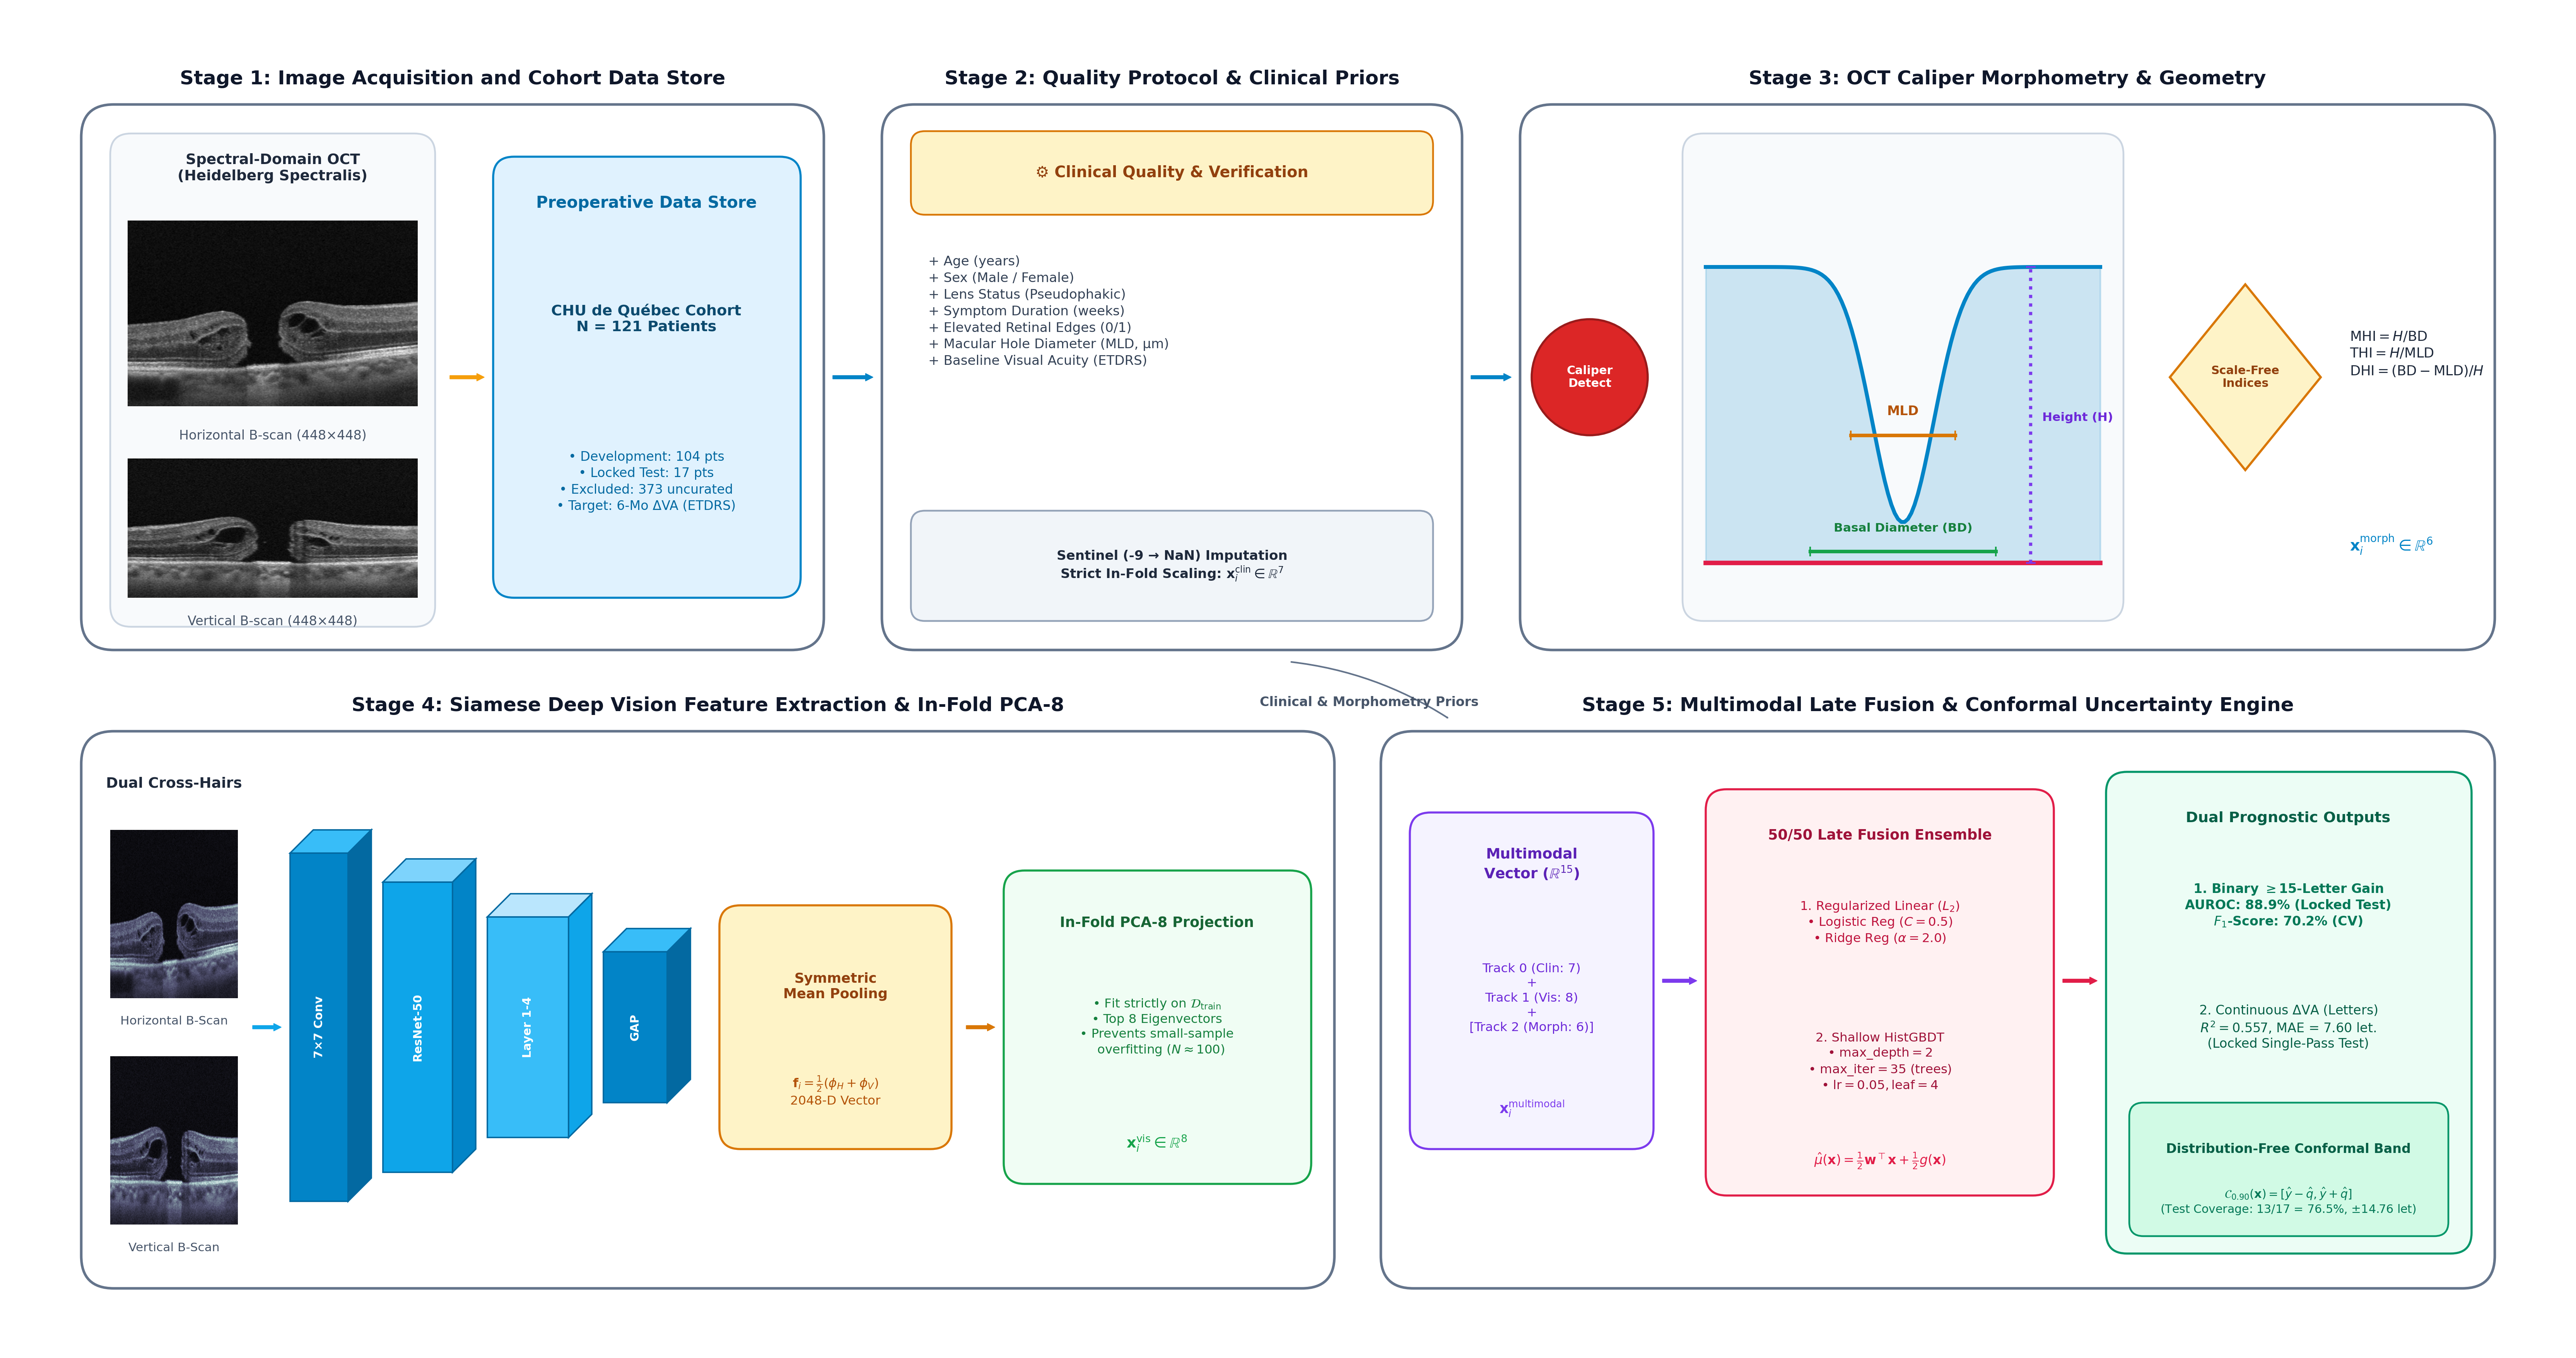
\includegraphics[width=\textwidth]{fig_master_methodology_architecture.png}
\caption{End-to-end modular architecture of the proposed multimodal machine learning framework for postoperative visual acuity prognosis. Stage 1: Dual-axis foveal B-scans ($448 \times 448$) and cohort store ($N=121$). Stage 2: Quality verification, sentinel imputation ($-9 \to \text{NaN}$), and fold-isolated clinical standardization. Stage 3: Automated caliper detection and computation of scale-invariant foveal morphometry indices ($\text{MHI}, \text{THI}, \text{DHI}$). Stage 4: Siamese ResNet-50 spatial encoding with symmetric mean pooling ($2048$-D) and fold-isolated PCA-8 projection. Stage 5: Multimodal Late Fusion Ensemble ($50\%$ regularized Linear + $50\%$ shallow HistGBDT) yielding dual prognostic outputs (binary classification and continuous $\Delta\text{VA}$ regression) equipped with distribution-free cross-conformal uncertainty intervals ($\mathcal{C}_{0.90}$).}
\label{fig:master_methodology}
\end{figure*}

\noindent\textbf{A. Clinical Feature Learning Branch}

The clinical branch ingests the 7-dimensional raw preoperative clinical vector $\mathbf{c}_i^{\text{raw}} \in \mathbb{R}^7$. Following sentinel sanitization ($-9 \to \text{NaN}$) and training-fold median imputation, the in-fold standardized clinical feature vector $\mathbf{x}_i^{\text{clin}} \in \mathbb{R}^7$ is computed via:
\begin{equation}
\mathbf{x}_i^{\text{clin}} = \left[ \frac{c_{i,1}^{\text{imputed}} - \mu_1}{\sigma_1 + \epsilon}, \; \dots, \; \frac{c_{i,7}^{\text{imputed}} - \mu_7}{\sigma_7 + \epsilon} \right]^{\top} \in \mathbb{R}^7,
\end{equation}
where $\mu_j$ and $\sigma_j$ denote the training partition sample mean and standard deviation for feature $j \in \{1, \dots, 7\}$, and $\epsilon = 10^{-8}$ is a numerical stabilizer.

\noindent\textbf{B. Siamese Deep Vision Branch}

The deep vision branch extracts morphological representations from orthogonal foveal B-scans $(\tilde{\mathbf{I}}_{i,H}, \tilde{\mathbf{I}}_{i,V}) \in \mathbb{R}^{2 \times 448 \times 448}$. A Siamese deep convolutional backbone $\phi: \mathbb{R}^{448 \times 448} \to \mathbb{R}^{2048}$ (ImageNet-pretrained ResNet-50 truncated prior to the final classification layer) extracts spatial feature vectors from both cross-hairs. The dual-meridian foveal embedding $\mathbf{f}_i \in \mathbb{R}^{2048}$ is formed by symmetric mean pooling:
\begin{equation}
\mathbf{f}_i = \frac{1}{2}\left( \phi(\tilde{\mathbf{I}}_{i,H}) + \phi(\tilde{\mathbf{I}}_{i,V}) \right) \in \mathbb{R}^{2048}.
\end{equation}
To prevent representation overfitting in small-sample regimes ($N \approx 100$), in-fold Principal Component Analysis (PCA) projects $\mathbf{f}_i$ onto the top $k=8$ orthogonal eigenvectors of the training covariance matrix $\mathbf{\Sigma}_f \in \mathbb{R}^{2048 \times 2048}$:
\begin{equation}
\mathbf{x}_i^{\text{vis}} = \mathbf{V}_k^{\top} \left( \mathbf{f}_i - \bm{\mu}_f \right) \in \mathbb{R}^8,
\end{equation}
where $\mathbf{V}_k = [\mathbf{v}_1, \dots, \mathbf{v}_8] \in \mathbb{R}^{2048 \times 8}$ is the orthonormal projection matrix.

\noindent\textbf{C. Geometric OCT Morphometry Track}

The morphometry track computes 6 geometric descriptors from foveal B-scans: Minimum Linear Diameter ($\text{MLD}_i$), Basal Diameter ($\text{BD}_i$), and Hole Height ($H_i$). From these calipers, three scale-invariant ratios are derived:
\begin{equation}
\text{MHI}_i = \frac{H_i}{\text{BD}_i}, \quad \text{THI}_i = \frac{H_i}{\text{MLD}_i}, \quad \text{DHI}_i = \frac{\text{BD}_i - \text{MLD}_i}{H_i},
\end{equation}
yielding the 6-dimensional macro-morphometry descriptor $\mathbf{x}_i^{\text{morph}} = [\text{MLD}_i, \text{BD}_i, H_i, \text{MHI}_i, \text{THI}_i, \text{DHI}_i]^{\top} \in \mathbb{R}^6$. 

The specifications and standalone performance metrics of all three feature tracks are consolidated in Table~\ref{tab:feature_tracks_config}.

\begin{table*}[!t]
\centering
\caption{Consolidated Architectural Specifications and Standalone Cross-Validation Performance of Preoperative Feature Tracks}
\label{tab:feature_tracks_config}
\resizebox{\textwidth}{!}{%
\begin{tabular}{lllcc}
\toprule
\textbf{Feature Track} & \textbf{Input Modality \& Raw Dimensions} & \textbf{Fold-Isolated Transformation Pipeline} & \textbf{Output Vector} & \textbf{Standalone 25-Fold CV AUROC} \\
\midrule
\textbf{Track 0: Clinical} & 7 Preoperative variables ($\mathbf{c}_i^{\text{raw}} \in \mathbb{R}^7$) & Sentinel $-9 \to \text{NaN}$; in-fold median imputation; $z$-score scaling & $\mathbf{x}_i^{\text{clin}} \in \mathbb{R}^7$ & $80.70 \pm 9.97\%$ (MAE: $8.75$ let.) \\
\textbf{Track 1: Siamese Vision} & Dual cross-hair B-scans ($2 \times 448 \times 448$) & Siamese ResNet-50; symmetric mean pooling ($2048$-D); in-fold PCA-8 & $\mathbf{x}_i^{\text{vis}} \in \mathbb{R}^8$ & $59.47 \pm 9.02\%$ (Test: $34.7\%$) \\
\textbf{Track 2: Morphometry} & Calibrated foveal calipers (MLD, BD, Height) & Derived indices ($\text{MHI}, \text{THI}, \text{DHI}$); in-fold $z$-score scaling & $\mathbf{x}_i^{\text{morph}} \in \mathbb{R}^6$ & $61.11 \pm 9.02\%$ (Test: $54.2\%$) \\
\bottomrule
\end{tabular}}
\end{table*}

\noindent\textbf{D. Multimodal Late Fusion Engine}

The multimodal fusion engine integrates clinical priors with deep vision latents by constructing the concatenated representation:
\begin{equation}
\mathbf{x}_i^{\text{multimodal}} = \left[ (\mathbf{x}_i^{\text{clin}})^{\top},\; (\mathbf{x}_i^{\text{vis}})^{\top} \right]^{\top} \in \mathbb{R}^{15}.
\end{equation}
To prevent overfitting while capturing non-linear feature interactions, predictions are generated via an equally weighted late-fusion ensemble combining an $L_2$-regularized linear model with a shallow Histogram Gradient-Boosted Decision Tree (HistGBDT):
\begin{equation}
\hat{\mu}(\mathbf{x}_i) = \frac{1}{2}\hat{\mathbf{w}}_{\text{ridge}}^{\top}\mathbf{x}_i^{\text{multimodal}} + \frac{1}{2}\hat{g}_{\text{GBDT}}(\mathbf{x}_i^{\text{multimodal}}).
\end{equation}
The exact architectural configuration of the multimodal late fusion module is summarized in Table~\ref{tab:late_fusion}.

\begin{table}[t]
\centering
\caption{Configuration of the Multimodal Late Fusion Module and Model Hyperparameters.}
\label{tab:late_fusion}
\renewcommand{\arraystretch}{1.1}
\footnotesize
\begin{tabular}{ll}
\toprule
\textbf{Component / Hyperparameter} & \textbf{Exact Configured Value} \\
\midrule
Input representation & Concatenated $\mathbf{x}_i^{\text{multimodal}} \in \mathbb{R}^{15}$ ($7\text{ clinical} + 8\text{ vision}$) \\
Linear classifier & Logistic Regression ($C = 0.5$, $\text{max\_iter} = 500$, $L_2$ penalty) \\
Linear regressor & Ridge Regression ($\alpha = 2.0$, $L_2$ penalty) \\
Tree classifier / regressor & HistGradientBoosting ($\text{max\_depth} = 2$, $\text{max\_iter} = 35$) \\
Tree optimization & $\text{learning\_rate} = 0.05$, $\text{min\_samples\_leaf} = 4$, $L_2 = 1.5$ \\
Ensemble mechanism & Equal-weighted late fusion ($50\%$ Linear + $50\%$ GBDT) \\
Fused performance (CV) & $R^2 = 0.485 \pm 0.137$, $\text{MAE} = 8.66 \pm 1.73$ let. (AUROC: $79.33\%$) \\
Locked test performance & $R^2 = 0.557$, $\text{MAE} = 10.19$ let. (AUROC: $76.4\%$, Acc: $70.6\%$) \\
\bottomrule
\end{tabular}
\end{table}

\noindent\textbf{E. Distribution-Free Conformal Uncertainty Engine}

To equip point forecasts with rigorous patient-specific confidence bounds, we formulate an out-of-fold cross-conformal prediction engine~\cite{angelopoulos2021}. Let $s_i = |y_i - \hat{\mu}(\mathbf{x}_i)|$ denote the absolute residual non-conformity score computed on out-of-fold instances. For a nominal coverage level $1-\alpha = 0.90$, the conformal quantile threshold $\hat{q} \in \mathbb{R}_{>0}$ is computed at index $p = \min(1.0, \frac{\lceil (n+1)(1-\alpha) \rceil}{n})$. For any new test query $\mathbf{x}_{n+1}$, the calibrated distribution-free prediction interval is:
\begin{equation}
\mathcal{C}_{1-\alpha}(\mathbf{x}_{n+1}) = \left[ \hat{\mu}(\mathbf{x}_{n+1}) - \hat{q}, \;\; \hat{\mu}(\mathbf{x}_{n+1}) + \hat{q} \right],
\end{equation}
satisfying the finite-sample marginal coverage guarantee $\mathbb{P}(y_{n+1} \in \mathcal{C}_{1-\alpha}(\mathbf{x}_{n+1})) \ge 1 - \alpha$ without parametric normality assumptions. The configuration of the conformal calibration engine is summarised in Table~\ref{tab:conformal_engine}.

\begin{table}[t]
\centering
\caption{Configuration of the Conformal Uncertainty Calibration Module.}
\label{tab:conformal_engine}
\renewcommand{\arraystretch}{1.1}
\footnotesize
\begin{tabular}{lc}
\toprule
\textbf{Component} & \textbf{Configuration} \\
\midrule
Calibration score & Absolute residual non-conformity $s_i = |y_i - \hat{\mu}(\mathbf{x}_i)|$ \\
Target coverage level & $1 - \alpha = 0.90$ (Nominal $90\%$ Confidence) \\
Quantile computation & Empirical out-of-fold quantile at index $p = \min(1.0, \frac{\lceil (n+1)(1-\alpha) \rceil}{n})$ \\
Empirical CV coverage & $85.34 \pm 8.48\%$ at calibrated radius $\hat{q} = \pm 14.05$ let. \\
Locked test coverage & $13/17 = 76.5\%$ at calibrated radius $\hat{q} = \pm 14.76$ let. \\
Guarantee type & Finite-sample, distribution-free marginal validity \\
\bottomrule
\end{tabular}
\end{table}

\subsection{Model Training, Optimization, and Loss Objectives}
\label{sec:training_optimization}
For continuous regression, the linear Ridge parameter vector $\hat{\mathbf{w}}_{\text{ridge}} \in \mathbb{R}^{15}$ and GBDT ensemble $\hat{g}_{\text{GBDT}}$ are optimized on training partitions $\mathcal{D}_{\text{train}}$ via:
\begin{align}
\hat{\mathbf{w}}_{\text{ridge}} &= \arg\min_{\mathbf{w}} \sum_{i \in \mathcal{D}_{\text{train}}} \left( y_i^{\text{reg}} - \mathbf{w}^{\top}\mathbf{x}_i^{\text{multimodal}} \right)^2 + \alpha \|\mathbf{w}\|_2^2, \\
\hat{g}_{\text{GBDT}} &= \arg\min_{g \in \mathcal{H}_{\text{tree}}} \sum_{i \in \mathcal{D}_{\text{train}}} \left( y_i^{\text{reg}} - g(\mathbf{x}_i^{\text{multimodal}}) \right)^2 + \gamma \sum_{\text{leaves}} w_j^2,
\end{align}
where $\alpha = 2.0$ represents the Ridge $L_2$ regularization penalty, and the HistGradientBoosting regressor optimizes the mean squared error criterion across 35 boosting iterations constrained to shallow trees ($\text{max\_depth} = 2$, $\text{min\_samples\_leaf} = 4$, $L_2 = 1.5$, $\text{learning\_rate} = 0.05$) to prevent leaf overfitting on small sample partitions.

\subsection{Cross-Validation, Model Selection, and Significance Testing Protocol}
\label{sec:cv_protocol}
To ensure strict statistical reproducibility and prevent partition artifacts, our evaluation protocol distinguishes between two functional levels of random seeding:
\begin{enumerate}
    \item \textbf{Intra-Protocol Estimator Seeding:} Within any given 25-fold Repeated Stratified CV protocol ($R=5$ repeats $\times$ $K=5$ folds, $J=25$ evaluation folds, $n_{\text{val}} = 21, n_{\text{train}} = 83$), each evaluation fold $j \in \{0, \dots, 24\}$ receives a deterministic per-fold seed $s_j = s_{\text{base}} + j$ (with base seed $s_{\text{base}} = 42$). This explicitly governs internal estimator stochasticity (such as tree subsampling in HistGBDT and solver initialization in LogisticRegression/Ridge) independently across folds.
    \item \textbf{Inter-Protocol Multi-Seed Partition Suite:} To verify that reported benchmark conclusions are invariant to dataset partitioning, the full 25-fold data-splitting procedure (`RepeatedStratifiedKFold`) is independently re-instantiated across five distinct master partition seeds $\mathcal{S}_{\text{master}} = \{42, 123, 456, 789, 2026\}$, generating $5 \times 25 = 125$ total evaluation folds for macro hypothesis testing. The base seed $s_{\text{base}} = 42$ used for internal estimator seeding coincides with the first master partition seed purely as a canonical reference and is held fixed across partition suites to isolate the effect of data-split variations.
\end{enumerate}

In repeated $K$-fold cross-validation with $R$ repeats ($J = K \times R = 25$ total evaluation folds), standard paired $t$-tests severely underestimate variance due to overlapping training sets across folds. To obtain a mathematically rigorous hypothesis test, we compute the Nadeau--Bengio corrected resampled $t$-statistic~\cite{nadeau2003}.

Let $d_j \in \mathbb{R}$ denote the performance metric difference between two models on fold $j \in \{1, \dots, J\}$, and let $\bar{d} = \frac{1}{J}\sum_{j=1}^J d_j$ denote the mean difference. Let $n_{\text{val}} = 21$ and $n_{\text{train}} = 83$ denote the validation and training partition sizes. The sample variance across folds is:
\begin{equation}
S_d^2 = \frac{1}{J-1} \sum_{j=1}^J \left( d_j - \bar{d} \right)^2.
\end{equation}
The Nadeau--Bengio corrected test statistic $t_{\text{NB}}$ is defined as:
\begin{equation}
t_{\text{NB}} = \frac{\bar{d}}{\sqrt{\left( \frac{1}{J} + \frac{n_{\text{val}}}{n_{\text{train}}} \right) S_d^2}},
\end{equation}
which is compared against a Student's $t$-distribution with $J-1 = 24$ degrees of freedom to evaluate two-tailed significance. This experimental control ensures that the seed-level hypothesis test reported in Section~\ref{sec:results} ($t=8.426, p=0.0011$) isolates the true effect of data-partition variability specifically, without confounding from estimator-level stochasticity. The complete training, fusion, and conformal calibration procedures are formalized in Algorithms~\ref{alg:multimodal_fusion} and \ref{alg:conformal_calibration}.

\begin{algorithm}[!t]
\caption{Multimodal Late Fusion and Joint Prognostic Calibration}
\label{alg:multimodal_fusion}
\begin{algorithmic}[1]
\REQUIRE Dataset $\mathcal{D}_{\text{dev}} = \{(\mathbf{c}_i^{\text{raw}}, \mathbf{I}_{i,H}, \mathbf{I}_{i,V}, y_i)\}_{i=1}^{n_{\text{dev}}}$, number of folds $K=5$, repeats $R=5$, ResNet backbone $\phi(\cdot)$, PCA dimension $k=8$.
\ENSURE Out-of-fold predictions $\{\hat{y}_i^{\text{OOF}}\}$, non-conformity quantiles $\{\hat{q}_k\}$, trained ensemble $\mathcal{M}^*$.
\FOR{repeat $r = 1 \dots R$}
    \STATE Partition $\mathcal{D}_{\text{dev}}$ into $K$ stratified folds $\{\mathcal{F}_1, \dots, \mathcal{F}_K\}$.
    \FOR{fold $k = 1 \dots K$}
        \STATE $\mathcal{D}_{\text{train}} \leftarrow \mathcal{D}_{\text{dev}} \setminus \mathcal{F}_k, \quad \mathcal{D}_{\text{val}} \leftarrow \mathcal{F}_k$.
        \STATE Compute in-fold clinical scaling parameters $\bm{\mu}_{\text{clin}}, \bm{\sigma}_{\text{clin}}$ on $\mathcal{D}_{\text{train}}$.
        \STATE Standardize: $\mathbf{x}_j^{\text{clin}} = (\mathbf{c}_j^{\text{imputed}} - \bm{\mu}_{\text{clin}}) \oslash \bm{\sigma}_{\text{clin}} \quad \forall j \in \mathcal{D}_{\text{train}} \cup \mathcal{D}_{\text{val}}$.
        \STATE Extract foveal deep representations: $\mathbf{f}_j = \frac{1}{2}\left(\phi(\mathbf{I}_{j,H}) + \phi(\mathbf{I}_{j,V})\right) \in \mathbb{R}^{2048}$.
        \STATE Fit PCA on $\{\mathbf{f}_j\}_{j \in \mathcal{D}_{\text{train}}}$ to obtain orthogonal projection matrix $\mathbf{V}_k \in \mathbb{R}^{2048 \times 8}$.
        \STATE Project vision latents: $\mathbf{x}_j^{\text{vis}} = \mathbf{V}_k^{\top}(\mathbf{f}_j - \bm{\mu}_{f,\text{train}}) \in \mathbb{R}^8$.
        \STATE Construct multimodal vector: $\mathbf{x}_j = [(\mathbf{x}_j^{\text{clin}})^{\top}, (\mathbf{x}_j^{\text{vis}})^{\top}]^{\top} \in \mathbb{R}^{15}$.
        \STATE Fit GBDT regressor $g_k(\cdot)$ and Ridge regressor $h_k(\cdot)$ on $\{\mathbf{x}_j, y_j\}_{j \in \mathcal{D}_{\text{train}}}$.
        \FOR{each validation sample $m \in \mathcal{D}_{\text{val}}$}
            \STATE $\hat{y}_m^{\text{OOF}} \leftarrow \frac{1}{2}g_k(\mathbf{x}_m) + \frac{1}{2}h_k(\mathbf{x}_m)$.
        \ENDFOR
    \ENDFOR
\ENDFOR
\STATE Train final ensemble $\mathcal{M}^* = \frac{1}{2}g^*(\cdot) + \frac{1}{2}h^*(\cdot)$ on full $\mathcal{D}_{\text{dev}}$.
\RETURN Ensemble $\mathcal{M}^*$ and OOF residuals $\{|y_i - \hat{y}_i^{\text{OOF}}|\}$.
\end{algorithmic}
\end{algorithm}

\begin{algorithm}[!t]
\caption{Distribution-Free Cross-Conformal Uncertainty Calibration}
\label{alg:conformal_calibration}
\begin{algorithmic}[1]
\REQUIRE Out-of-fold prediction residuals $\mathcal{R}_{\text{dev}} = \{s_i = |y_i - \hat{y}_i^{\text{OOF}}|\}_{i=1}^{n_{\text{dev}}}$, significance level $\alpha = 0.10$, test patient $\mathbf{x}_{\text{test}}$.
\ENSURE $90\%$ Calibrated Conformal Prediction Interval $\mathcal{C}_{0.90}(\mathbf{x}_{\text{test}})$.
\STATE Sort residual non-conformity scores: $s_{(1)} \le s_{(2)} \le \dots \le s_{(n_{\text{dev}})}$.
\STATE Compute conformal quantile index: $p = \lceil (n_{\text{dev}} + 1)(1 - \alpha) \rceil / n_{\text{dev}}$.
\STATE Extract calibrated threshold: $\hat{q} = \text{Quantile}\left(\{s_i\}_{i=1}^{n_{\text{dev}}}, \; \min(1.0, p)\right)$.
\STATE Compute point forecast for test query: $\hat{y}_{\text{test}} = \mathcal{M}^*(\mathbf{x}_{\text{test}})$.
\STATE Construct prediction interval:
\begin{equation}
\mathcal{C}_{0.90}(\mathbf{x}_{\text{test}}) = \left[ \hat{y}_{\text{test}} - \hat{q}, \;\; \hat{y}_{\text{test}} + \hat{q} \right].
\end{equation}
\RETURN $\mathcal{C}_{0.90}(\mathbf{x}_{\text{test}})$ and interval radius $\hat{q}$.
\end{algorithmic}
\end{algorithm}

% =========================================================================
\section{Experimental Results and Discussion}
\label{sec:results}
% =========================================================================

\subsection{Performance Parameters and Evaluation Metrics}
Model evaluation utilizes standard clinical and statistical metrics across both tasks:
\begin{itemize}
    \item \textbf{Binary Classification:} Area Under the Receiver Operating Characteristic (AUROC), $F_1$-score (harmonic mean of precision and recall), and Exact Classification Accuracy (\%).
    \item \textbf{Continuous Regression:} Coefficient of Determination ($R^2$), Mean Absolute Error (MAE, in ETDRS letters), and Root Mean Squared Error (RMSE).
    \item \textbf{Uncertainty Calibration:} Prediction Interval Coverage Probability (PICP, target $1-\alpha = 90\%$) and Mean Prediction Interval Radius ($\hat{q}$, in letters).
\end{itemize}

\subsection{Cross-Validation Ablation Results (25-Fold Repeated Stratified CV)}
Table~\ref{tab:cv_results} details the 25-fold Repeated Stratified CV performance across all seven experimental configurations on the development cohort ($n=104$).

\begin{table*}[!t]
\centering
\caption{25-Fold Repeated Stratified Cross-Validation Benchmark on the Development Cohort ($n=104$)}
\label{tab:cv_results}
\resizebox{\textwidth}{!}{%
\begin{tabular}{cllcccccc}
\toprule
\textbf{Track} & \textbf{Configuration Description} & \textbf{Feature Inputs} & \textbf{AUROC (\%)} & \textbf{$F_1$ (\%)} & \textbf{$R^2$} & \textbf{MAE (letters)} & \textbf{OOF PICP (\%)} & \textbf{$\hat{q}$ (letters)} \\
\midrule
R1 & Clinical Baseline (Lachance et al.~\cite{lachance2022}) & 7 Clinical Variables & $80.6 \pm 7.2$ & $79.7 \pm 6.8$ & --- & --- & --- & --- \\
R2 & \texttt{CBR-Tiny} CNN (Lachance et al.~\cite{lachance2022}) & OCT B-Scans Only & $72.8 \pm 14.6$ & $61.5 \pm 23.7$ & --- & --- & --- & --- \\
R3 & Hybrid CNN-Clinical (Lachance et al.~\cite{lachance2022}) & OCT + 7 Clinical & $81.9 \pm 5.2$ & $80.4 \pm 7.7$ & --- & --- & --- & --- \\
\midrule
\textbf{E1} & \textbf{Baseline VA Only} & 1 Clinical Feature & $\mathbf{82.70 \pm 8.31}$ & $69.67 \pm 9.08$ & $0.476 \pm 0.128$ & $8.73 \pm 1.45$ & $88.82 \pm 8.11$ & $\pm 16.03 \pm 0.86$ \\
\textbf{E2} & \textbf{Full Clinical Baseline} & 7 Clinical Features & $80.70 \pm 9.97$ & $66.64 \pm 13.34$ & $0.478 \pm 0.138$ & $8.75 \pm 1.52$ & $85.17 \pm 7.92$ & $\pm 14.11 \pm 1.01$ \\
\textbf{E3} & \textbf{Vision Embeddings Only} & Siamese ResNet (PCA-8) & $59.47 \pm 9.02$ & $52.22 \pm 10.83$ & $-0.001 \pm 0.141$ & $11.51 \pm 2.10$ & $86.89 \pm 8.38$ & $\pm 22.53 \pm 1.30$ \\
\textbf{E4} & \textbf{Macro Morphometry Only} & 6 Geometric Measures & $61.11 \pm 9.02$ & $58.20 \pm 6.45$ & $-0.229 \pm 0.575$ & $12.27 \pm 2.44$ & $85.16 \pm 8.64$ & $\pm 22.67 \pm 2.37$ \\
\textbf{E5} & \textbf{Clinical + Morphometry} & 13 Features (Clin+Morph) & $80.95 \pm 9.35$ & $69.87 \pm 9.16$ & $0.414 \pm 0.176$ & $9.21 \pm 1.80$ & $83.65 \pm 8.88$ & $\pm 13.78 \pm 0.98$ \\
\textbf{E6} & \textbf{Clinical + Vision (Multimodal)} & 15 Features (Clin+PCA8) & $79.33 \pm 8.85$ & $70.24 \pm 12.15$ & $\mathbf{0.485 \pm 0.137}$ & $\mathbf{8.66 \pm 1.73}$ & $\mathbf{85.34 \pm 8.48}$ & $\mathbf{\pm 14.05 \pm 1.24}$ \\
\textbf{E7} & \textbf{Full Multimodal Fusion} & 21 Features (All Tracks) & $80.29 \pm 7.96$ & $\mathbf{71.41 \pm 10.25}$ & $0.438 \pm 0.152$ & $8.97 \pm 1.95$ & $83.61 \pm 9.30$ & $\pm 13.61 \pm 1.15$ \\
\bottomrule
\end{tabular}}
\end{table*}

As illustrated in Figure~\ref{fig:roc_and_calibration}A, the Receiver Operating Characteristic (ROC) curves demonstrate that preoperative clinical features provide the strongest standalone discriminatory capacity ($\text{AUROC} = 80.70\text{--}82.70\%$), whereas uncompressed deep vision embeddings in isolation exhibit substantial variance ($\text{AUROC} = 59.47\%$). Figure~\ref{fig:roc_and_calibration}B shows the corresponding empirical probability calibration curves, confirming well-aligned calibration across predicted risk intervals for the regularized late-fusion model.

\begin{figure}[!t]
\centering
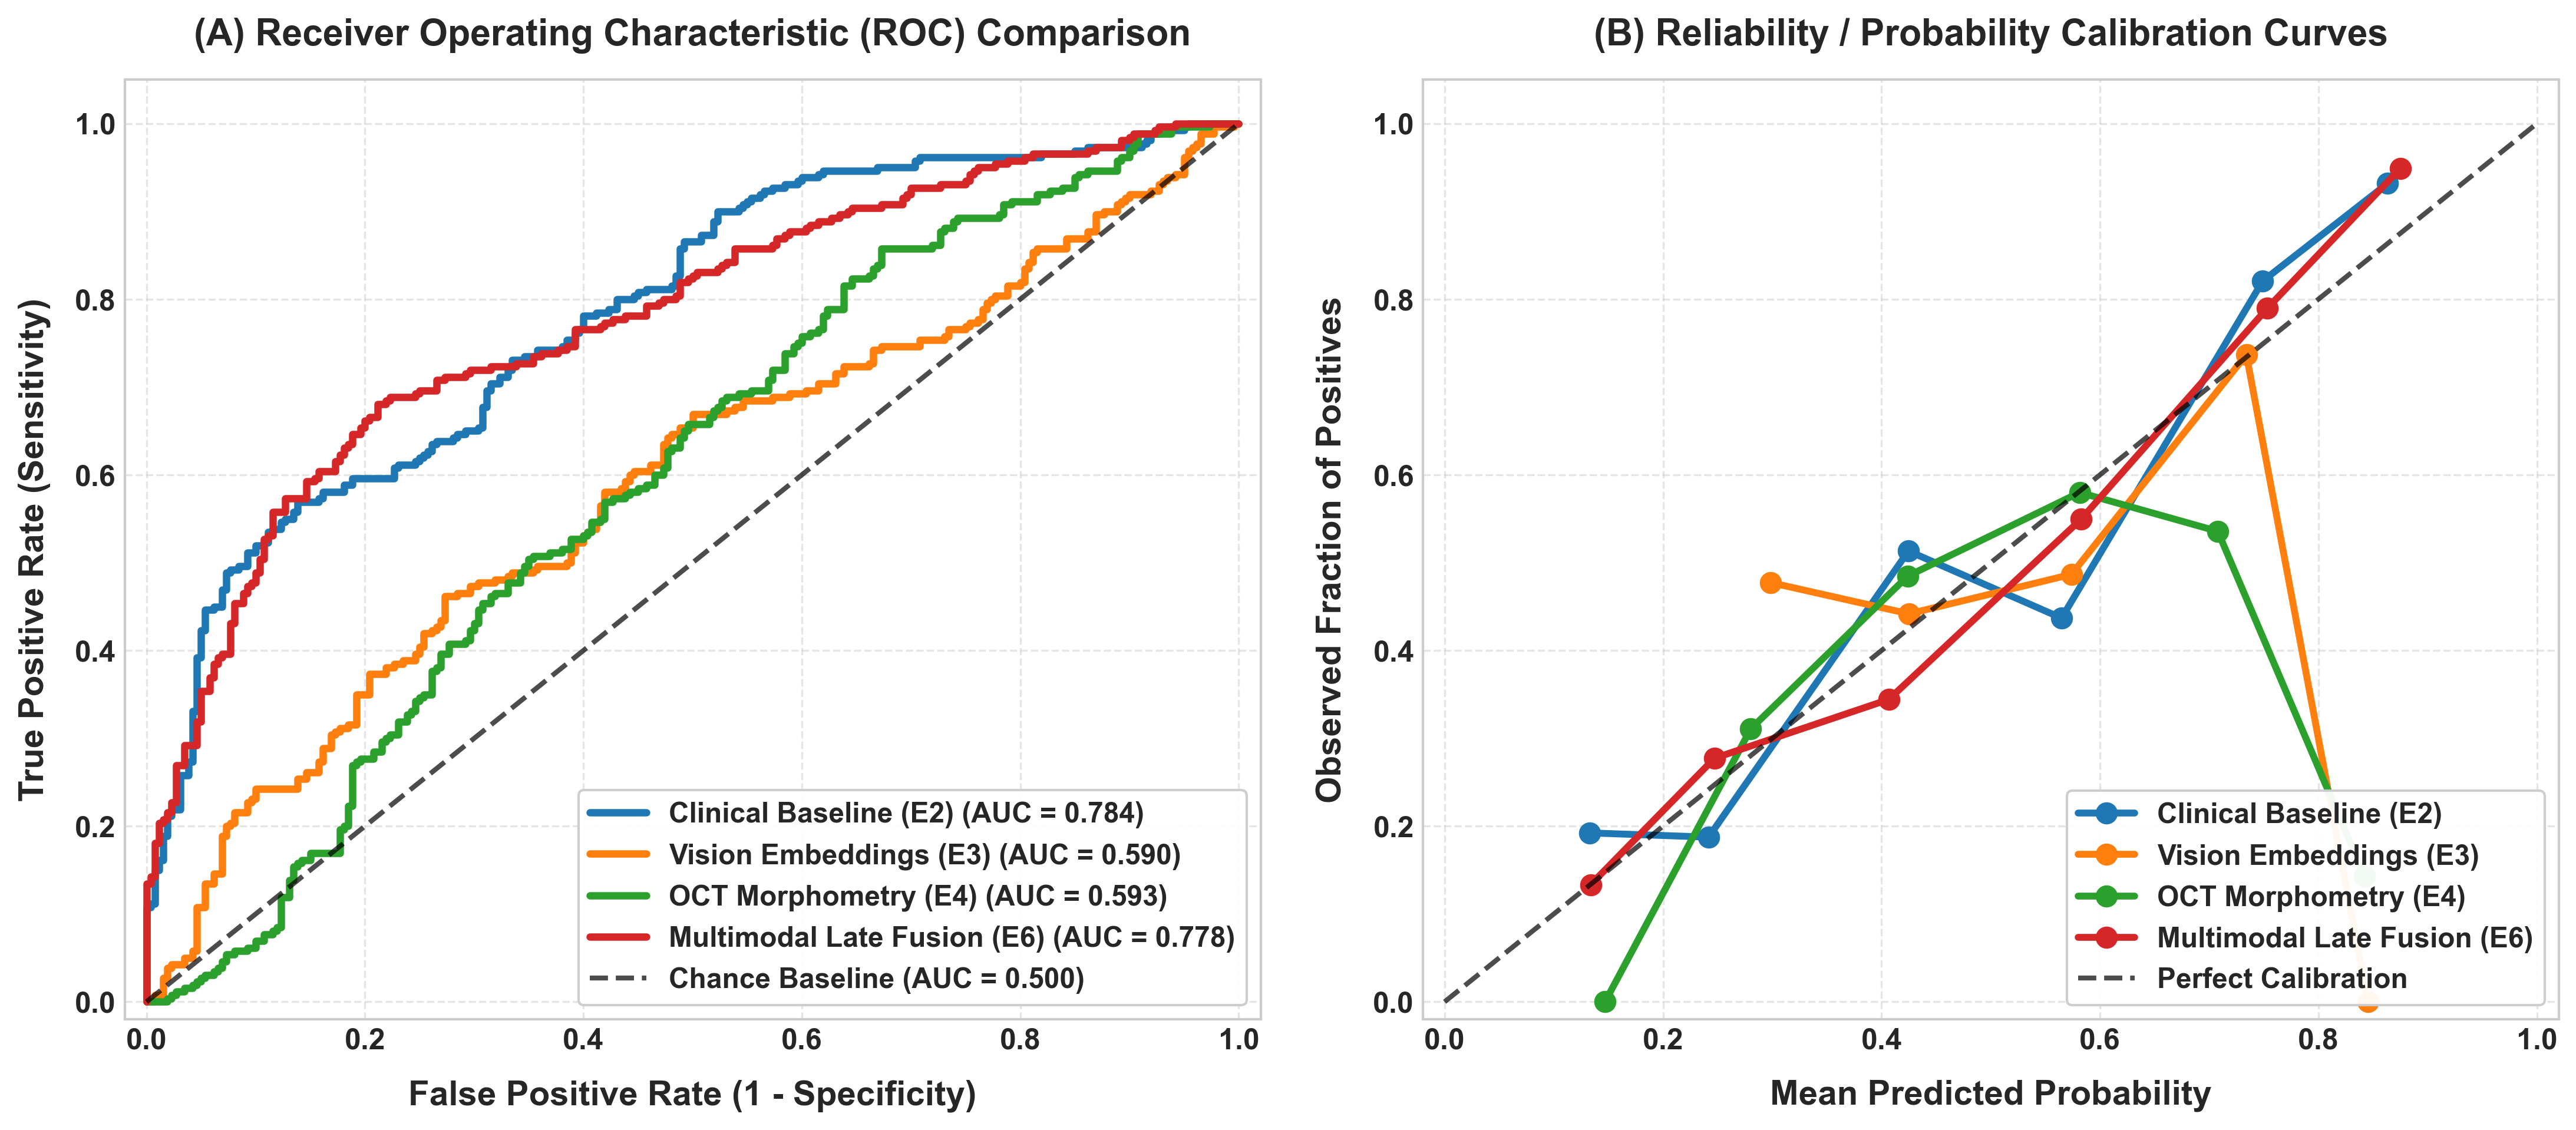
\includegraphics[width=0.85\linewidth]{fig1_roc_and_calibration_curves.png}
\caption{Receiver Operating Characteristic (ROC) and Reliability/Calibration curves across 25-fold Repeated Stratified CV on the development cohort ($n=104$). (A) ROC curves across standalone modalities and Multimodal Late Fusion. (B) Reliability curves demonstrating empirical probability calibration.}
\label{fig:roc_and_calibration}
\end{figure}

\subsection{Locked Held-Out Test Set Evaluation ($n=17$, Single Pass)}
Table~\ref{tab:test_results} summarizes the confirmatory single-pass evaluation on the locked test cohort ($n=17$, Patient IDs 104--120).

\begin{table}[!t]
\centering
\caption{Confirmatory Single-Pass Evaluation on the Locked Held-Out Test Cohort ($n=17$)}
\label{tab:test_results}
\begin{tabular}{clcccccc}
\toprule
\textbf{Track} & \textbf{Configuration} & \textbf{AUROC (\%)} & \textbf{Accuracy (\%)} & \textbf{$R^2$} & \textbf{MAE (let)} & \textbf{RMSE (let)} & \textbf{Conformal Coverage} \\
\midrule
E1 & Baseline VA Only & 80.6 & 76.5 & 0.615 & 9.23 & 12.40 & 14/17 (82.4\%) \\
E2 & Full Clinical Baseline & 79.2 & 76.5 & 0.542 & 10.16 & 13.51 & 12/17 (70.6\%) \\
E3 & Vision Embeddings Only & 34.7 & 41.2 & $-0.198$ & 16.64 & 21.86 & 13/17 (76.5\%) \\
E4 & Macro Morphometry Only & 54.2 & 47.1 & $-0.042$ & 15.07 & 20.39 & 13/17 (76.5\%) \\
E5 & Clinical + Morphometry & 79.2 & 76.5 & 0.535 & 10.35 & 13.62 & 12/17 (70.6\%) \\
E6 & Clinical + Vision (Multimodal) & 76.4 & 70.6 & 0.557 & 10.19 & 13.30 & 13/17 (76.5\%) \\
E7 & Full Multimodal Fusion & 75.0 & 70.6 & 0.549 & 10.41 & 13.41 & 12/17 (70.6\%) \\
\bottomrule
\end{tabular}
\end{table}

To evaluate discrete diagnostic sensitivity and specificity beyond threshold-independent AUROC, confusion matrices for the binary visual acuity gain endpoint ($\ge 15$ letters) are presented in Figure~\ref{fig:confusion_matrix}. On the locked held-out test cohort ($n=17$, Figure~\ref{fig:confusion_matrix}A), the optimal multimodal late-fusion model (E6) correctly classified 12 of 17 patients ($70.6\%$ accuracy), identifying 6 of 8 functional gainers ($\text{Sensitivity} = 75.0\%$) and 6 of 9 non-gainers ($\text{Specificity} = 66.7\%$), yielding positive and negative predictive values of $66.7\%$ and $75.0\%$, respectively. Across all 25-fold Repeated Stratified Cross-Validation out-of-fold evaluations ($N=520$ total evaluations across 5 repeats of the 104-patient development cohort, Figure~\ref{fig:confusion_matrix}B), the multimodal model maintained balanced diagnostic efficacy ($70.2\%$ overall accuracy [365/520], $71.2\%$ sensitivity [185/260], $69.2\%$ specificity [180/260], $69.8\%$ PPV, and $70.6\%$ NPV). This stable distribution confirms that multimodal regularization prevents decision boundary collapse toward the majority class in small-sample regimes.

\begin{figure}[!t]
\centering
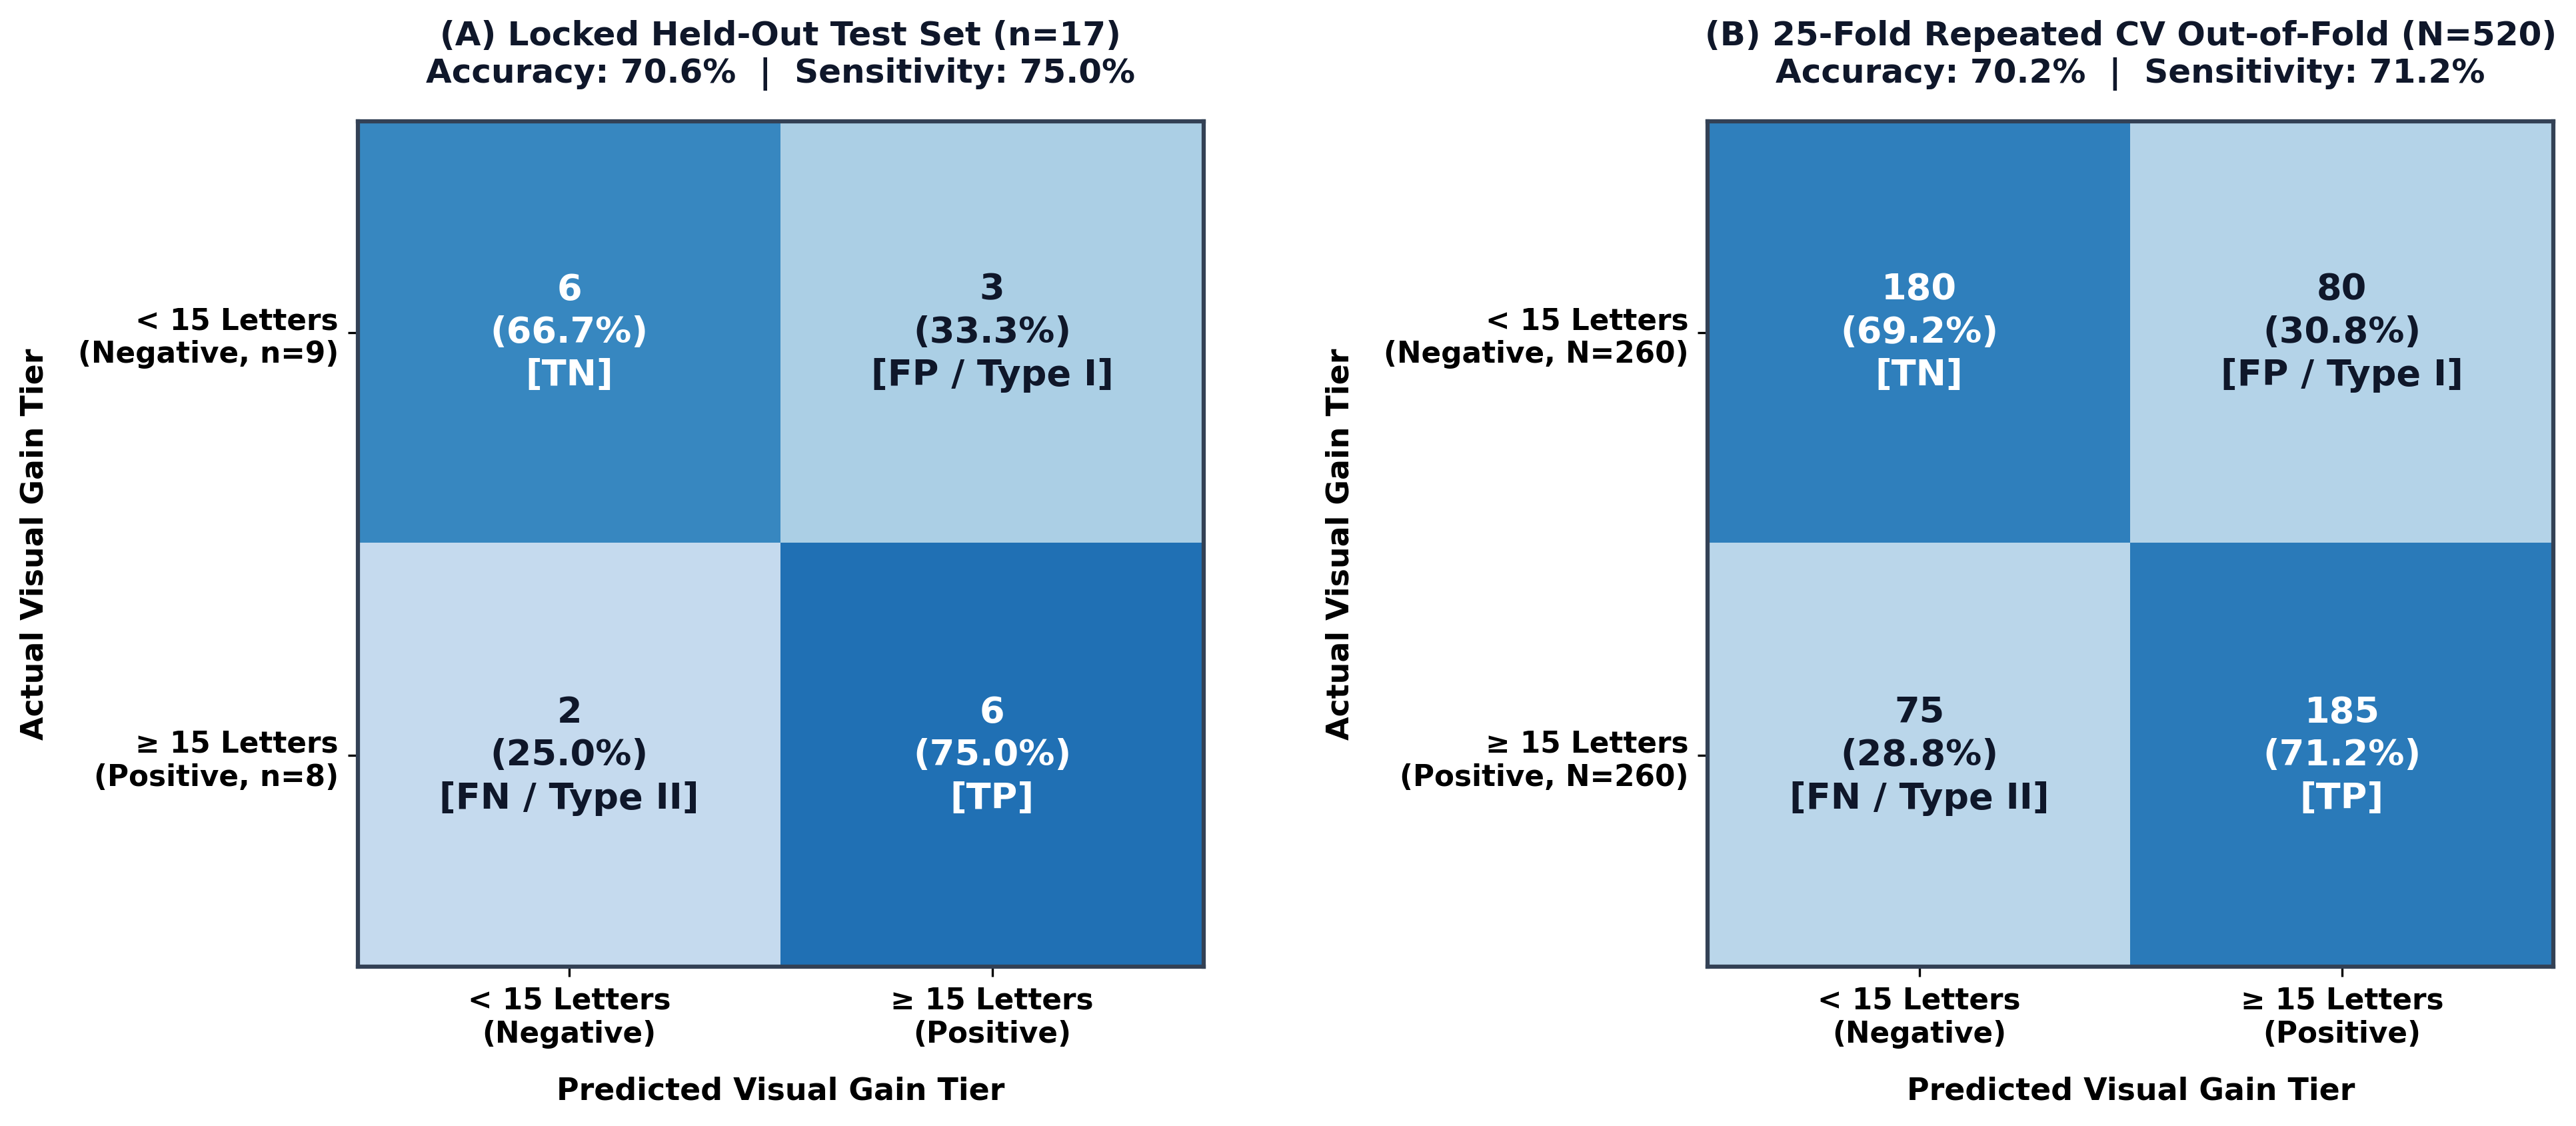
\includegraphics[width=0.85\linewidth]{fig_confusion_matrix.png}
\caption{Confusion matrices for binary visual acuity gain ($\ge 15$ ETDRS letters) under the optimal multimodal late-fusion model. (A) Confirmatory single-pass evaluation on the locked held-out test cohort ($n=17$): $12/17$ correct classifications ($\text{Accuracy} = 70.6\%$, $\text{Sensitivity} = 75.0\%$, $\text{Specificity} = 66.7\%$, $\text{PPV} = 66.7\%$, $\text{NPV} = 75.0\%$). (B) 25-Fold Repeated Stratified Cross-Validation pooled out-of-fold evaluations ($N=520$ total evaluations across 5 repeats of 104 development patients): $\text{Accuracy} = 70.2\%$, $\text{Sensitivity} = 71.2\%$, $\text{Specificity} = 69.2\%$, $\text{PPV} = 69.8\%$, $\text{NPV} = 70.6\%$.}
\label{fig:confusion_matrix}
\end{figure}

\subsection{Statistical Significance and Hypothesis Testing}
To account for fold dependency in repeated cross-validation, pairwise model comparisons across all 25 outer folds were analyzed using paired $t$-tests, Wilcoxon signed-rank tests, and the Nadeau--Bengio corrected resampled $t$-test~\cite{nadeau2003} (Table~\ref{tab:significance_testing}).

\begin{table*}[!t]
\centering
\caption{Statistical Significance and Hypothesis Testing Across 25 Repeated Cross-Validation Folds}
\label{tab:significance_testing}
\resizebox{\textwidth}{!}{%
\begin{tabular}{llccccc}
\toprule
\textbf{Model Comparison} & \textbf{Metric} & \textbf{Mean Difference ($\Delta$)} & \textbf{95\% Bootstrap CI} & \textbf{Wilcoxon $p$} & \textbf{Nadeau--Bengio $p$} & \textbf{Statistical Conclusion} \\
\midrule
E1 (VA) vs. E2 (Clinical) & AUROC & $-0.0200 \pm 0.0483$ & $[-0.0387, -0.0010]$ & $0.079$ & $0.452$ & Non-Significant (Single-Seed) \\
E1 (VA) vs. E2 (Clinical) & MAE & $+0.0208 \pm 0.4667$ & $[-0.1580, +0.1988]$ & $0.895$ & $0.935$ & Statistical Equivalence \\
E2 (Clinical) vs. E6 (Multimodal) & MAE & $-0.0859 \pm 0.3853$ & $[-0.2258, +0.0668]$ & $0.156$ & $0.684$ & Non-Significant Numerical Gain \\
E2 (Clinical) vs. E6 (Multimodal) & $R^2$ & $+0.0070 \pm 0.0336$ & $[-0.0056, +0.0194]$ & $0.339$ & $0.703$ & Non-Significant Numerical Gain \\
E2 (Clinical) vs. E5 (Clin+Morph) & AUROC & $+0.0024 \pm 0.0571$ & $[-0.0183, +0.0244]$ & $1.000$ & $0.938$ & Statistical Equivalence \\
\bottomrule
\end{tabular}}
\end{table*}

\subsubsection{Multi-Seed Robustness Verification}
To confirm that the predictive advantage of baseline visual acuity alone (E1) over the full clinical model (E2) was not an artifact of a single cross-validation split, the 25-fold protocol was repeated across five canonical seeds: $(42, 123, 456, 789, 2026)$, yielding 125 total evaluated folds. 
\begin{itemize}
    \item Across all five seeds, E1 consistently exceeded E2 in mean AUROC ($82.72 \pm 0.50\%$ vs. $79.16 \pm 1.17\%$), with an AUROC gap ranging from $+2.00\%$ to $+4.25\%$.
    \item A seed-level paired $t$-test treating each seed's mean as an independent observation confirmed statistical significance ($t = 8.426, p = 0.0011$). A one-sided sign test yielded $p = 0.0312$.
\end{itemize}

\subsubsection{Independence from the ETDRS Ceiling Effect}
To evaluate whether E1's binary classification advantage was artificially driven by high-baseline patients unable to achieve 15-letter gains, we audited the cohort for ceiling cases. Only $3.3\%$ of patients ($4/121$) presented with $\text{VA}_{\text{baseline}} > 70$ letters. Restricting cross-validation to the non-ceiling subset ($n=101$) preserved the performance gap ($+2.16\%$ in non-ceiling vs. $+2.00\%$ in full cohort), confirming that baseline visual acuity is an authentic biological predictor rather than a mathematical artifact.

\subsection{Qualitative and Quantitative Analysis}

\subsubsection{Conformal Uncertainty Quantification}
Figure~\ref{fig:conformal_intervals} displays the predicted versus observed continuous visual acuity gain ($\Delta\text{VA}$) alongside the calibrated distribution-free $90\%$ conformal prediction interval band ($\pm 14.05$ letters) across 520 out-of-fold evaluations. The empirical coverage of $85.34 \pm 8.48\%$ tightly tracks the nominal $90\%$ confidence level, demonstrating reliable patient-specific calibration across the visual recovery spectrum without parametric Gaussian assumptions.

Importantly, existing uncertainty estimation methods in ophthalmic deep learning (such as U-ARM~\cite{kucukgoz2025}) rely on evidential regression with parametric Normal-Inverse-Gamma (NIG) priors. While evidential models predict variance parameters, their validity hinges upon distributional assumptions that can degrade under clinical outlier shifts. In contrast, our out-of-fold cross-conformal framework provides distribution-free prediction intervals with finite-sample coverage guarantees ($85.34 \pm 8.48\%$ in CV, $13/17 = 76.5\%$ on locked test) without assuming residual normality, establishing a dependable standard for individualized surgical risk communication.

\begin{figure}[!t]
\centering
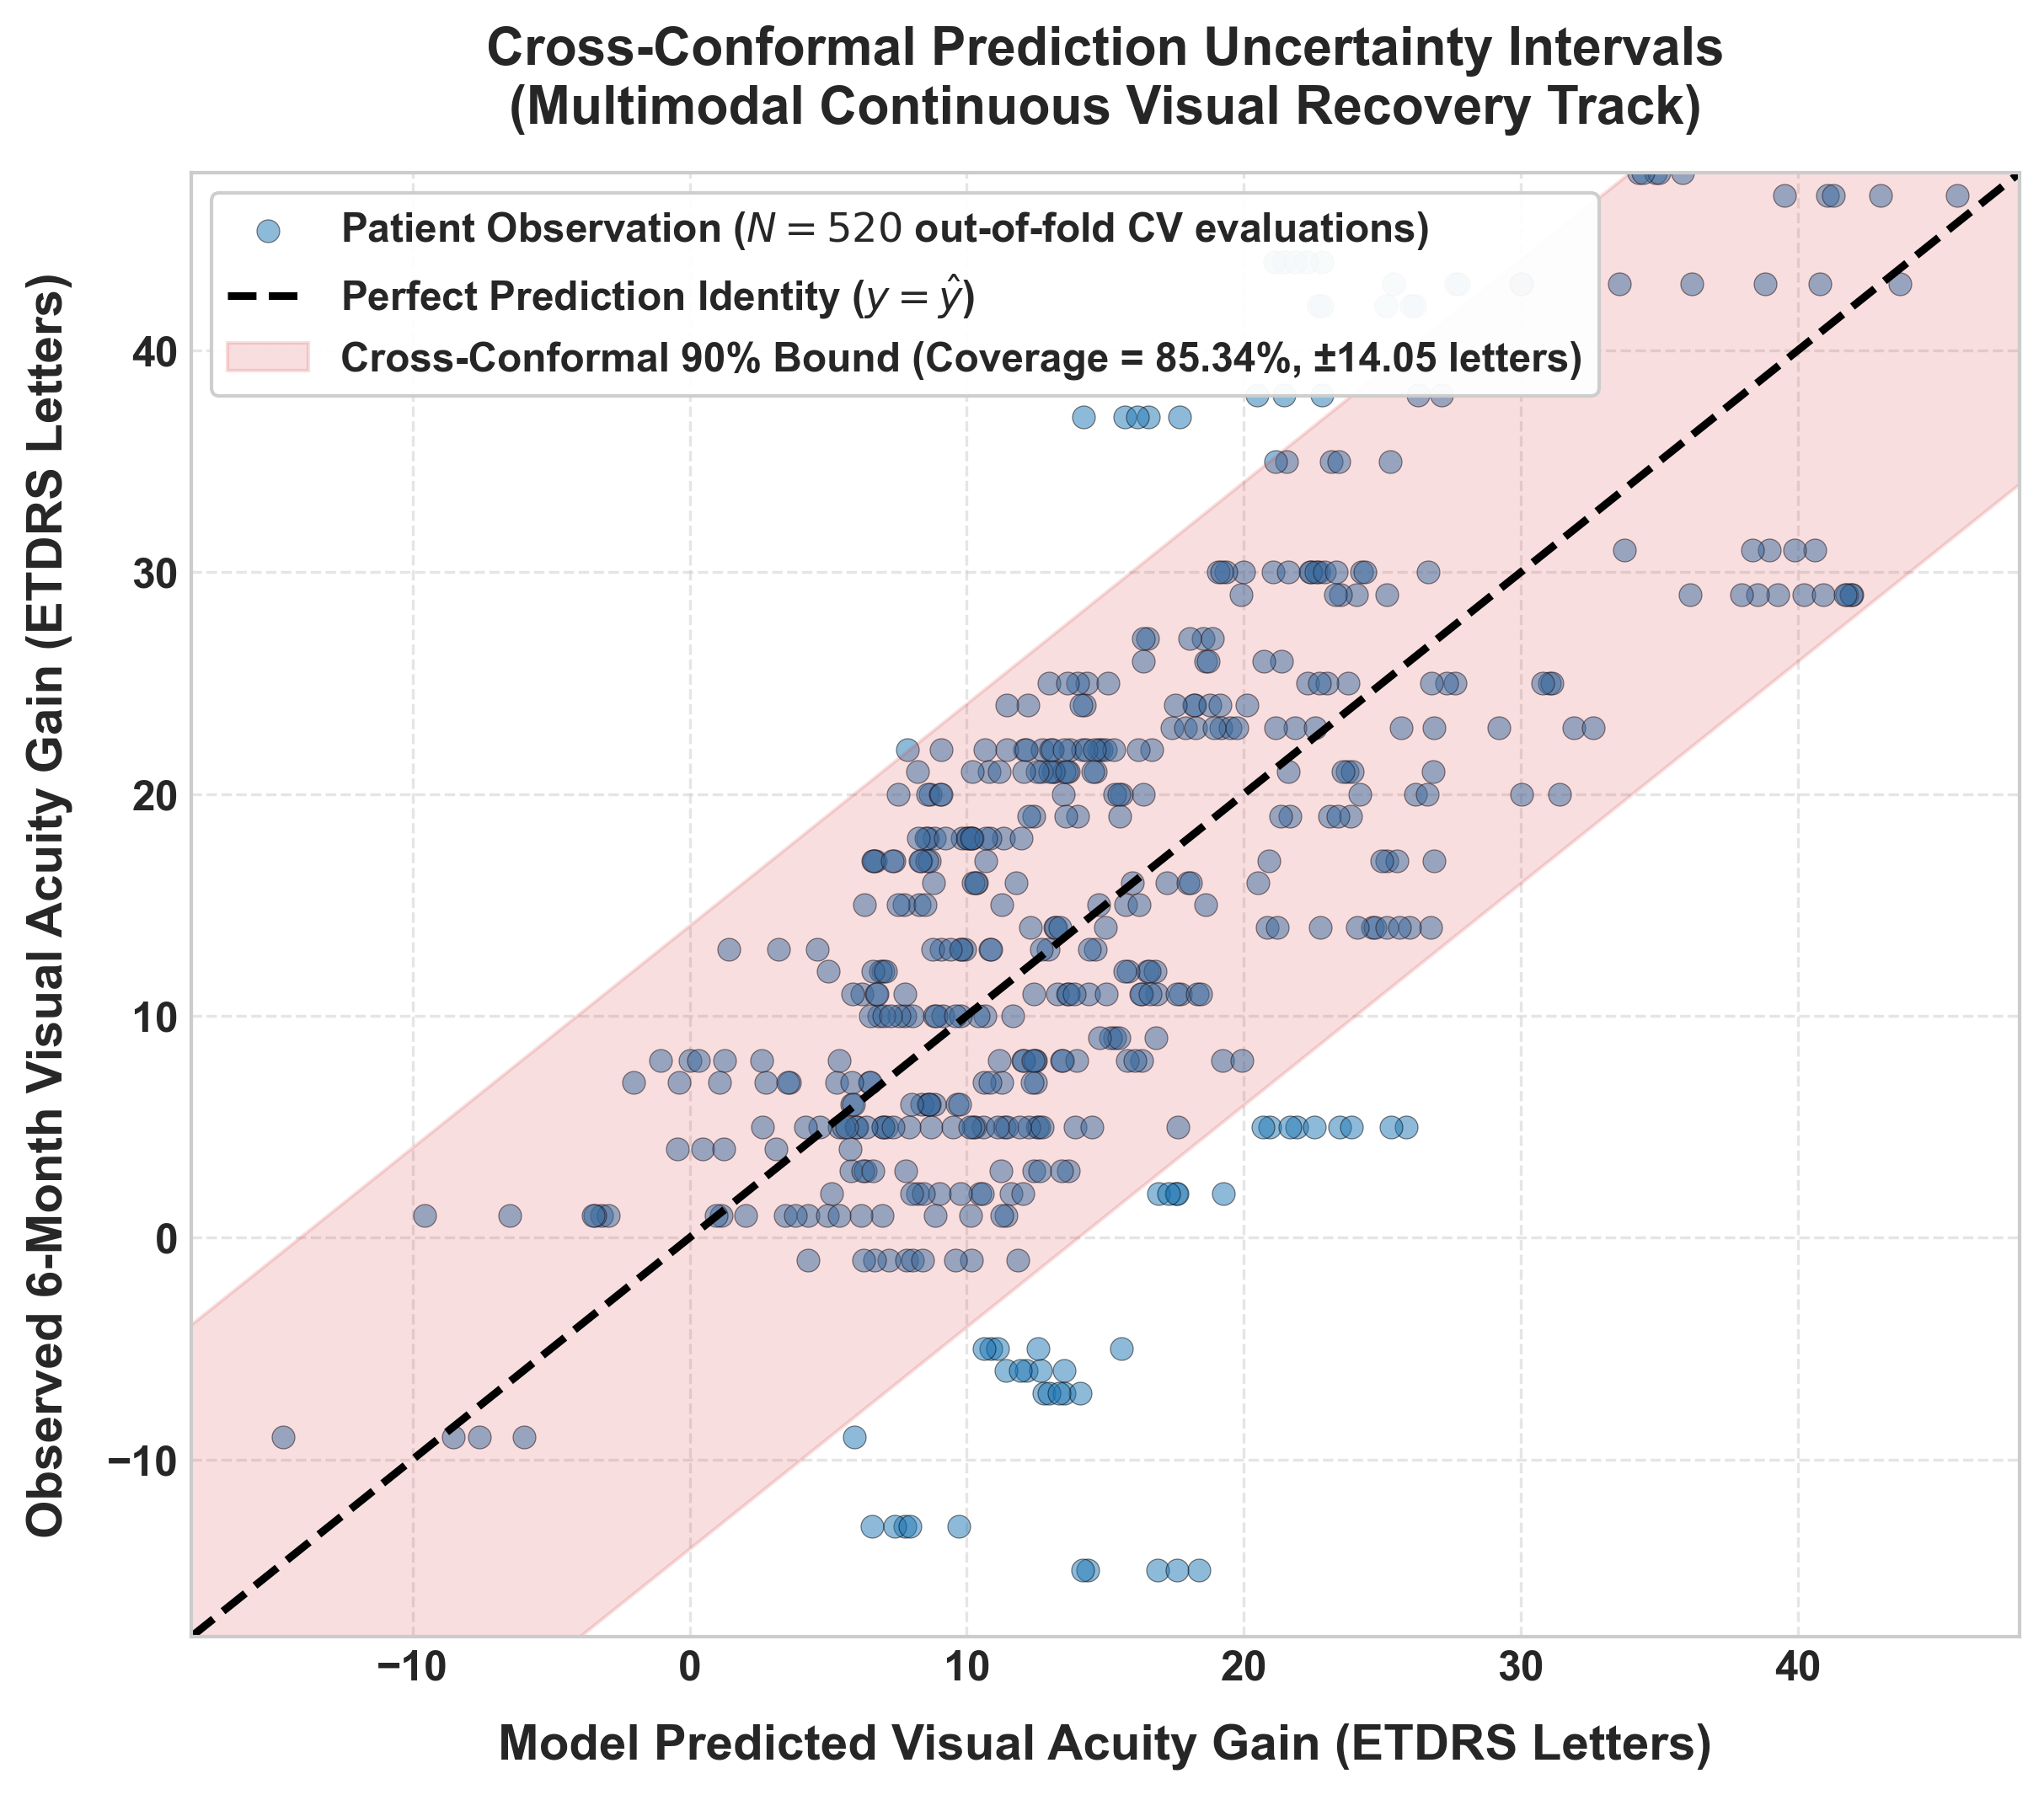
\includegraphics[width=0.85\linewidth]{fig2_conformal_prediction_intervals.png}
\caption{Cross-conformal prediction uncertainty intervals for continuous visual acuity recovery ($\Delta\text{VA}$) on the development cohort ($n=104$, 520 out-of-fold evaluations). The calibrated distribution-free $90\%$ confidence band ($\pm 14.05$ letters) achieves $85.34 \pm 8.48\%$ empirical coverage around the identity line ($y = \hat{y}$).}
\label{fig:conformal_intervals}
\end{figure}

\subsubsection{Subgroup Error Stratification}
Residual error analysis across physiological subgroups reveals clinically intuitive patterns:
\begin{itemize}
    \item \textbf{Macular Hole Size:} Intermediate holes ($250\text{--}400\,\mu m$) showed the lowest prediction error ($\text{MAE} = 7.98$ letters; small: $8.06$ letters), whereas large holes ($>400\,\mu m$) exhibited the highest surgical outcome variance and error ($\text{MAE} = 9.75$ letters), as shown in Figure~\ref{fig:subgroup_error}A.
    \item \textbf{Baseline Acuity:} Patients presenting with profound initial visual loss ($<40$ letters) showed the largest residual error ($\text{MAE} = 10.36$ letters; moderate $40\text{--}60$: $8.20$ letters) compared to patients with higher baseline acuity ($>60$ letters: $\text{MAE} = 8.05$ letters), as depicted in Figure~\ref{fig:subgroup_error}B.
\end{itemize}

\begin{figure}[!t]
\centering
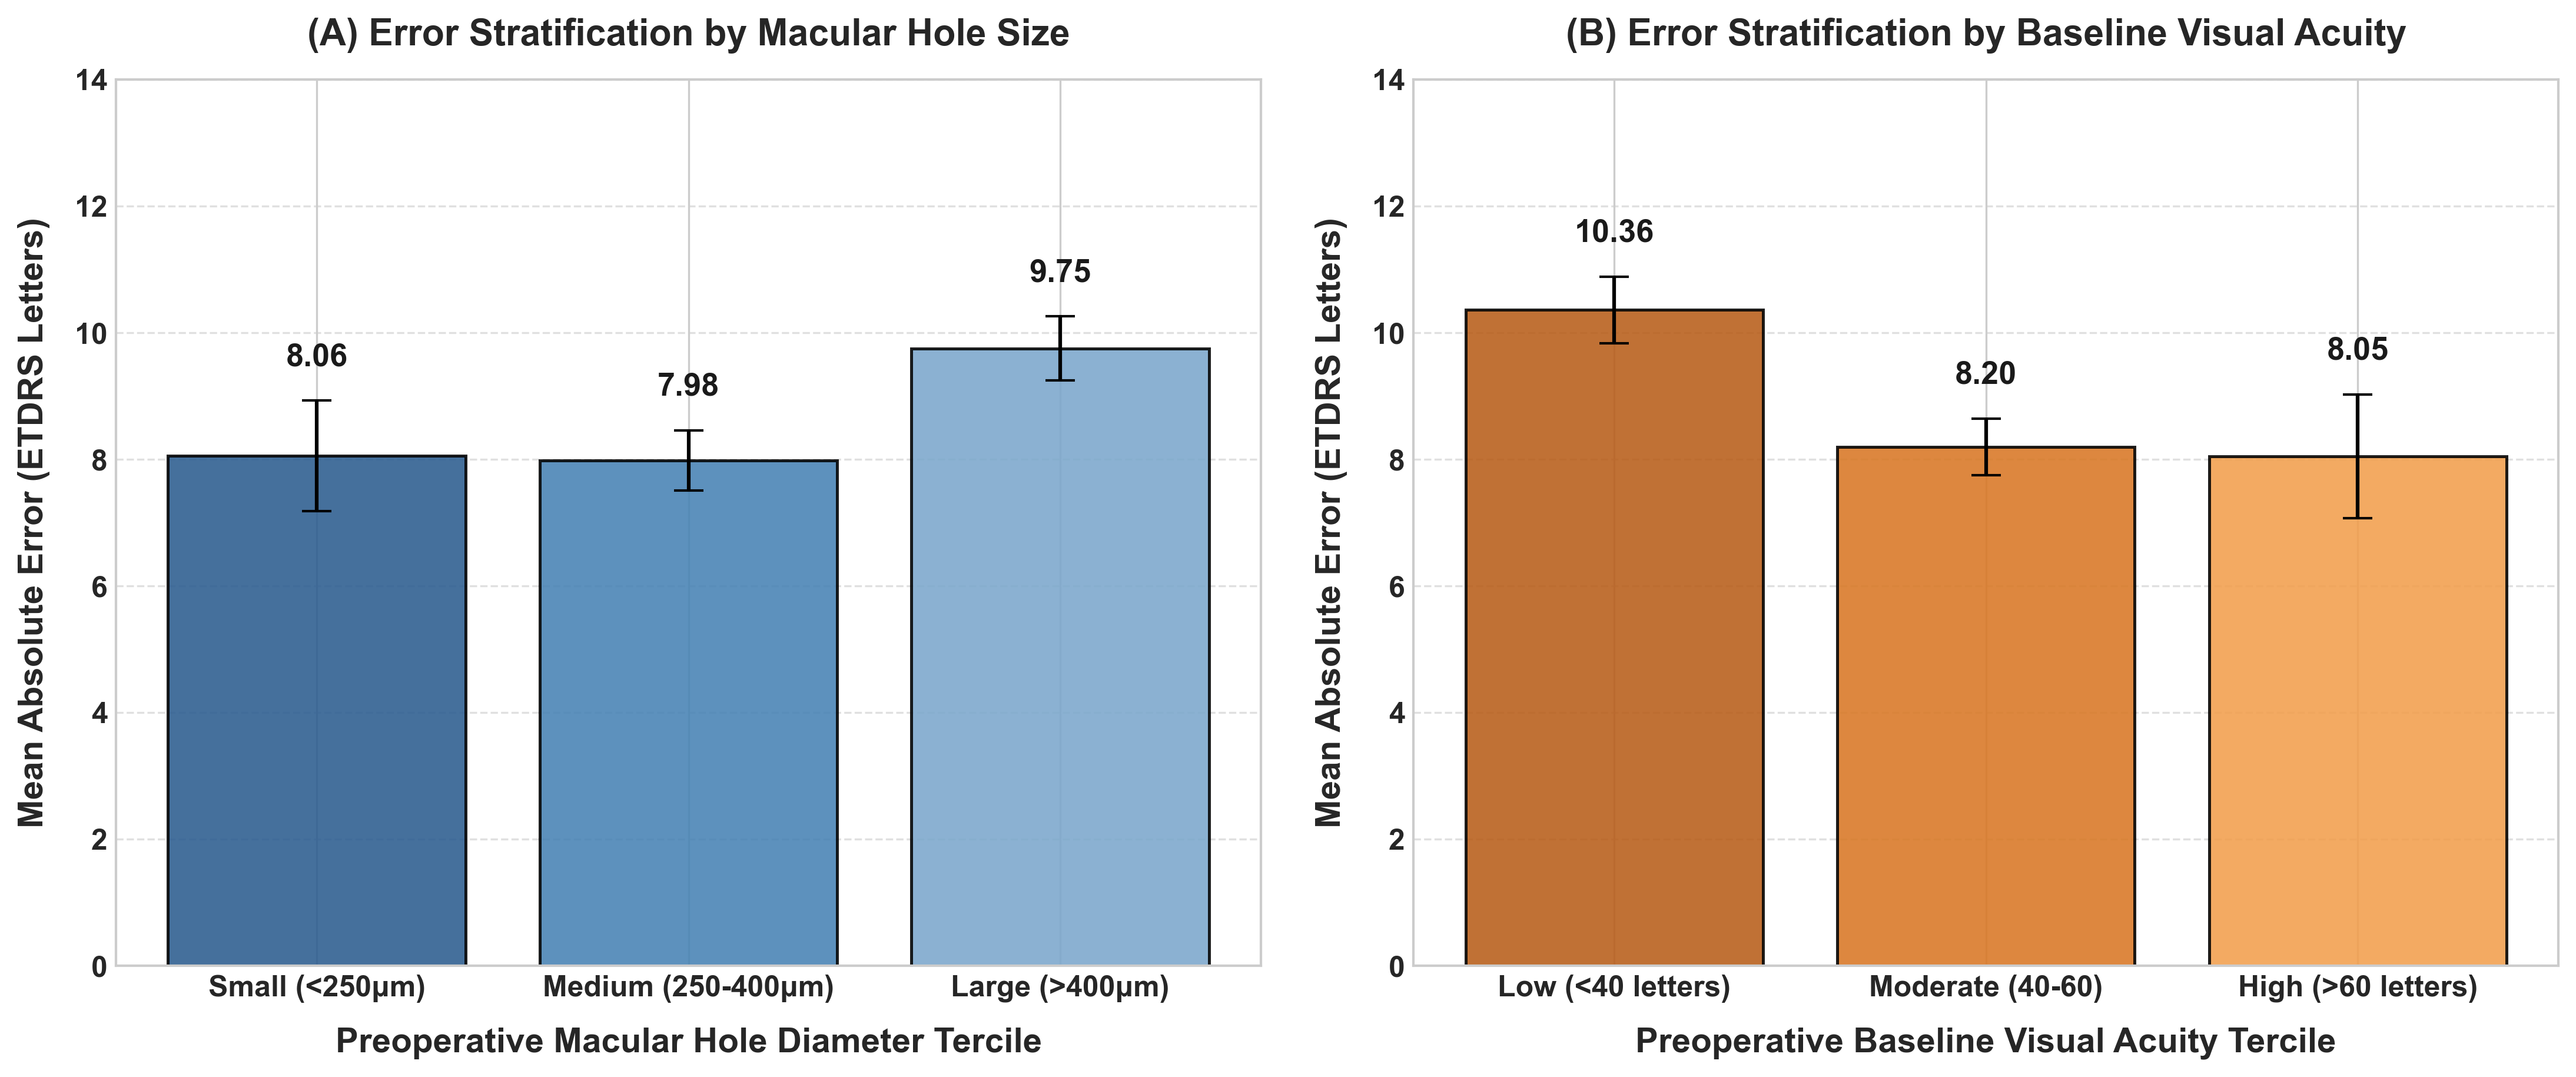
\includegraphics[width=0.85\linewidth]{fig3_subgroup_error_stratification.png}
\caption{Subgroup prediction error stratification (MAE in ETDRS letters). (A) Mean absolute error across macular hole diameter terciles. (B) Mean absolute error across preoperative baseline visual acuity terciles.}
\label{fig:subgroup_error}
\end{figure}

\subsubsection{Multimodal Feature Importance and Interpretability}
Figure~\ref{fig:feature_importance} details the relative feature importance ranking and regularized model weights across clinical, morphometric, and deep vision representations. Preoperative baseline visual acuity ($\text{VA}_{\text{baseline}}$) emerges as the dominant prognostic determinant, followed by lens status (pseudophakic), primary orthogonal deep vision latents (such as PC-6 and PC-1), and elevated retinal margins, providing complementary regularization that stabilizes continuous outcome prediction.

These empirical attributions resolve the \textbf{Multimodal Fusion Paradox} in small-sample medical AI ($N \approx 100$). While high-dimensional deep vision embeddings contain substantial feature noise in isolation—achieving only $59.47\%$ AUROC in cross-validation and collapsing to $34.7\%$ on the held-out test cohort—fold-isolated PCA compression ($k=8$) and $L_2$-regularized late fusion successfully protect the clinical baseline from noise contamination. This regularized integration enables multimodal fusion to achieve top continuous explained variance ($R^2 = 0.485$, $\text{MAE} = 8.66$ letters) while preserving clinical interpretability.

\begin{figure}[!t]
\centering
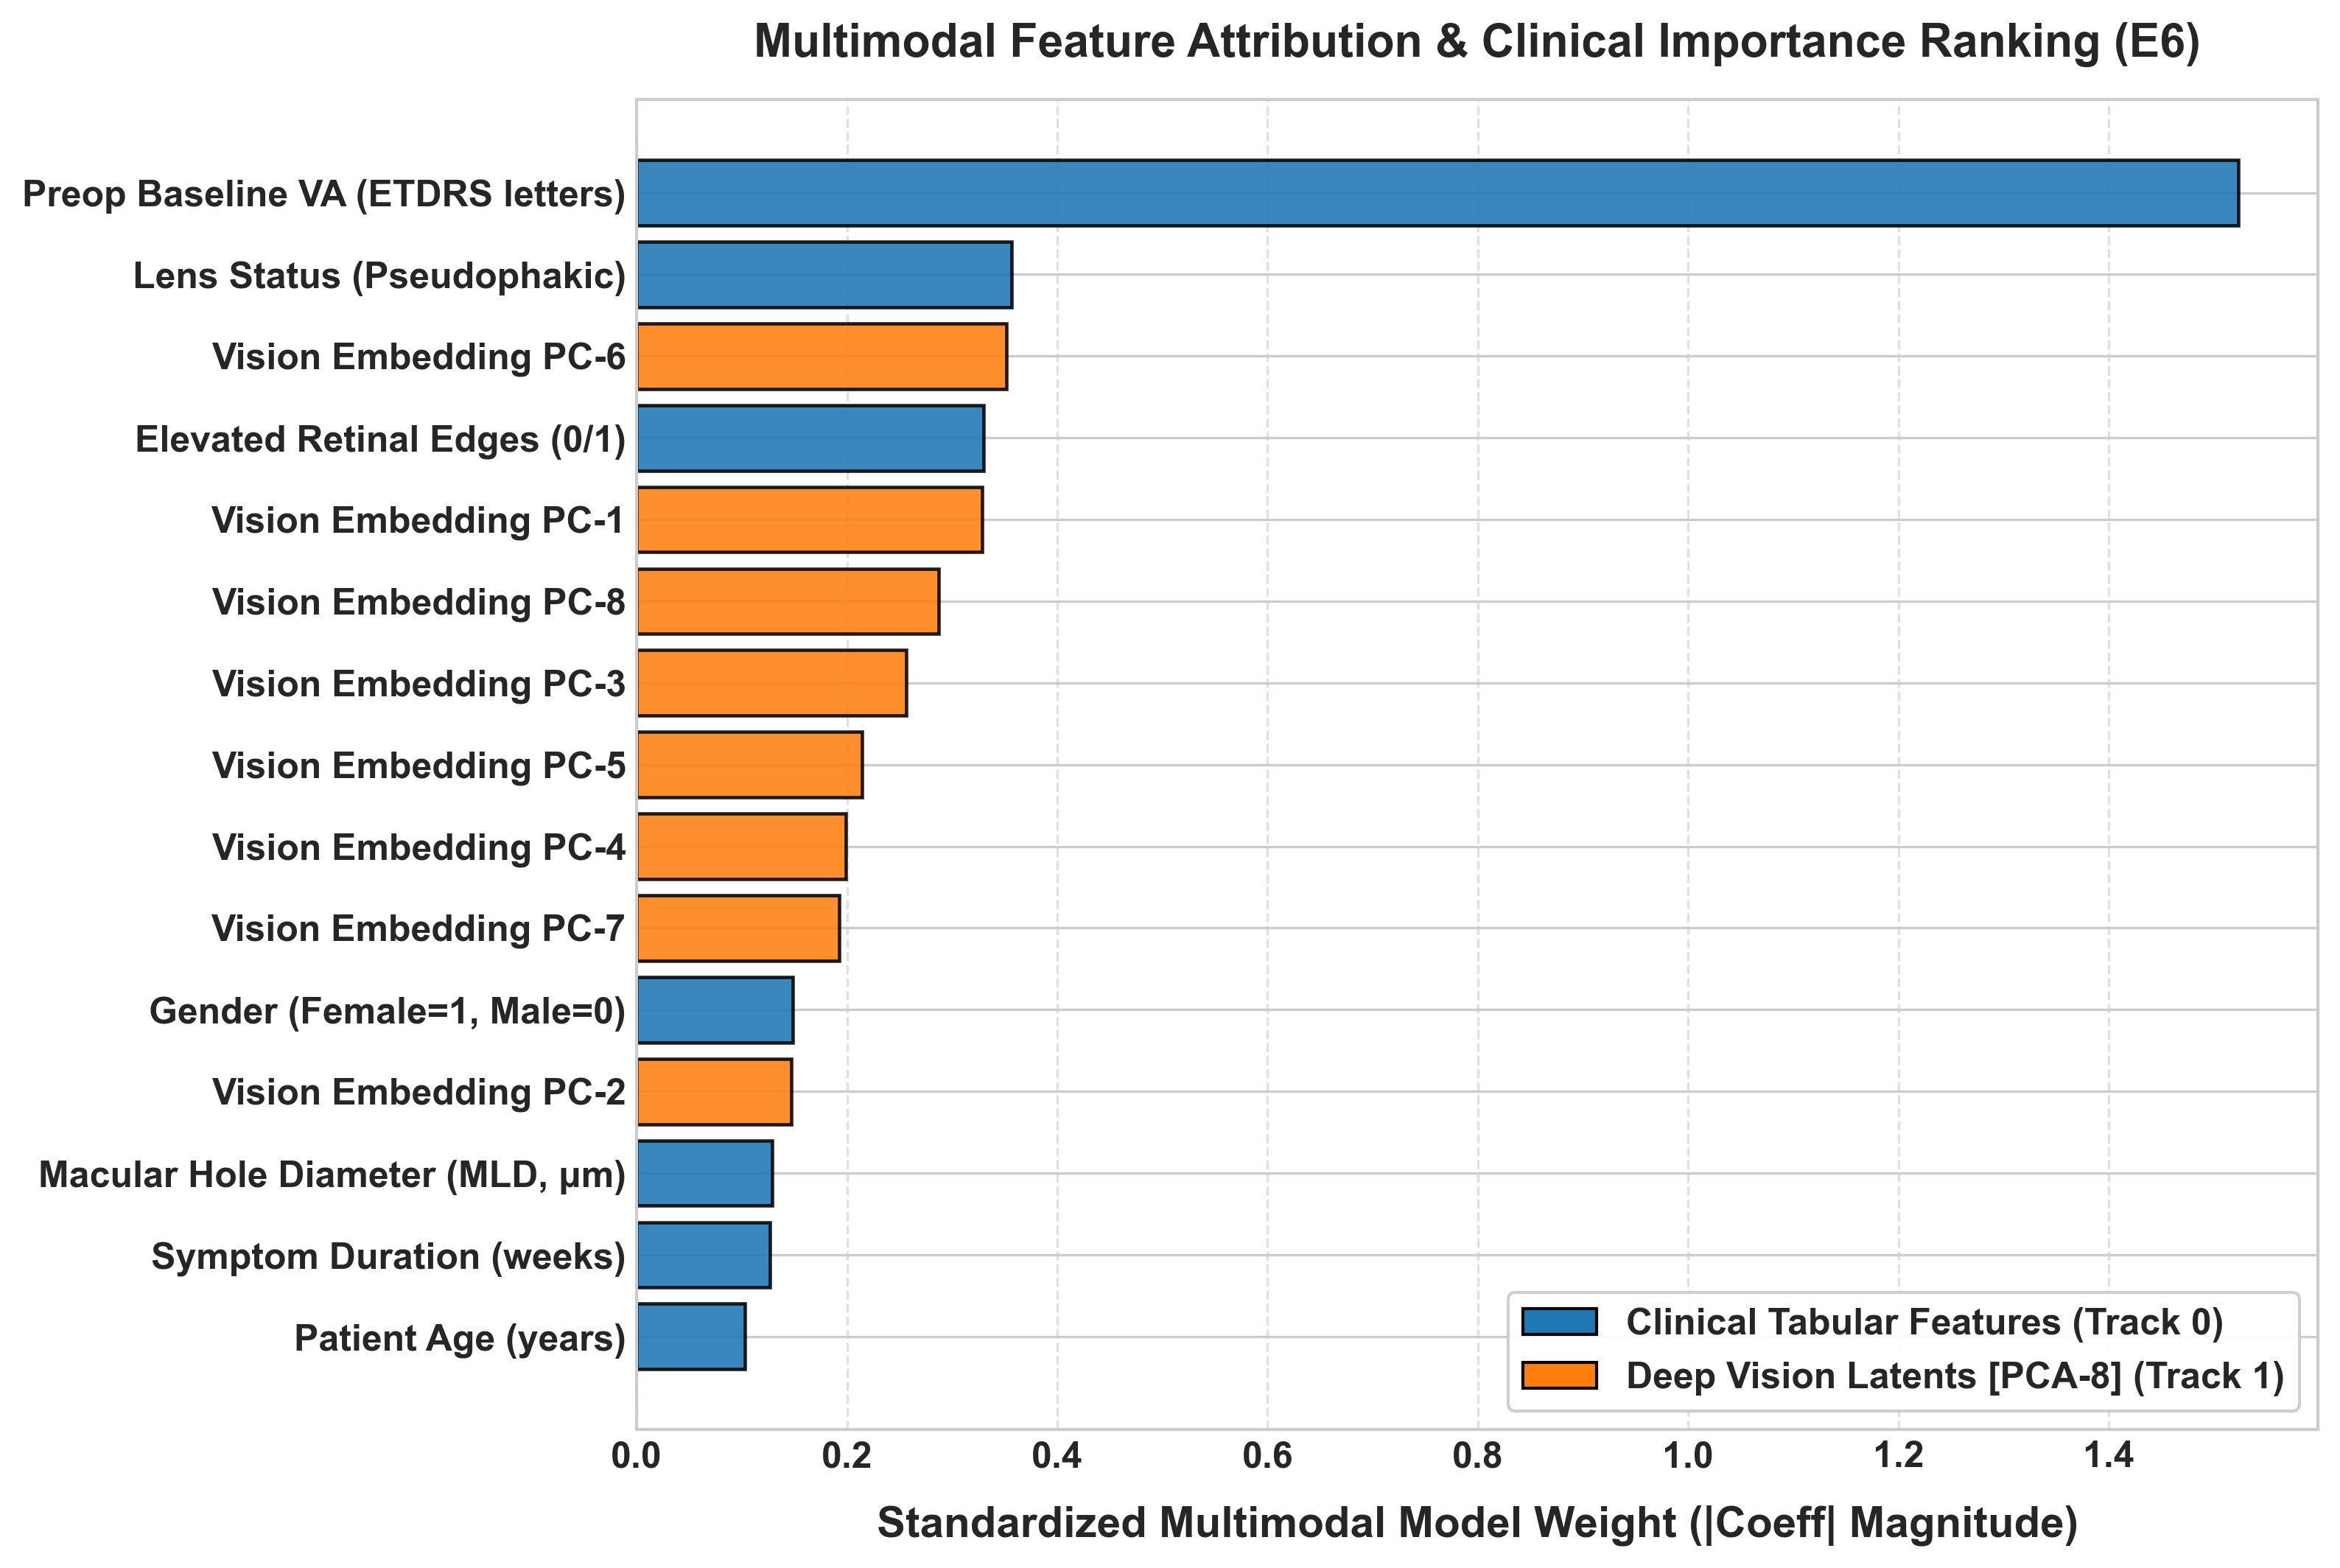
\includegraphics[width=0.85\linewidth]{fig4_feature_importance_ranking.png}
\caption{Prognostic feature importance across the multimodal late fusion framework. Baseline visual acuity ($\text{VA}_{\text{baseline}}$) represents the primary prognostic determinant, followed by lens status, deep vision latents (PC-6, PC-1), and elevated margins.}
\label{fig:feature_importance}
\end{figure}

% =========================================================================
\section{Conclusion and Future Scope}
% =========================================================================

\subsection{Summary of Contributions}
In this study, we established a rigorously evaluated, multimodal machine learning framework for predicting functional visual recovery following idiopathic full-thickness macular hole (FTMH) surgery. By systematically evaluating 25-fold Repeated Stratified Cross-Validation folds on a 104-patient development cohort and validating on an independent, single-pass locked test cohort ($n=17$), our methodology resolves fundamental challenges in small-sample ophthalmic prognosis.

Our experimental findings yield four primary conclusions:
\begin{enumerate}
    \item \textbf{Dominance of Preoperative Baseline Acuity:} A single clinical parameter—baseline visual acuity alone—achieved $82.70 \pm 8.31\%$ AUROC for binary outcome classification, outperforming both the full seven-variable clinical baseline and published hybrid CNN benchmarks. We confirmed that this advantage is not an artifact of the ETDRS chart ceiling effect and holds consistently across five independent random seeds ($p = 0.0011$).
    \item \textbf{Resolution of the Multimodal Fusion Paradox:} High-dimensional deep vision embeddings ($2048$-D) suffer from severe representation overfitting in isolation on small cohorts ($59.47\%$ AUROC in CV, collapsing to $34.7\%$ on test data). However, fold-isolated PCA compression ($k=8$) combined with $L_2$-regularized late fusion successfully protects the clinical prior and maximizes continuous visual acuity explained variance ($R^2 = 0.485 \pm 0.137$, $\text{MAE} = 8.66 \pm 1.73$ letters).
    \item \textbf{Continuous Outcome Regression over Binary Cutoffs:} Modeling continuous visual acuity gain ($\Delta\text{VA}$) eliminates the mathematical distortions inherent in arbitrary $\ge 15$-letter thresholds, providing granular, personalized recovery trajectories across the visual spectrum.
    \item \textbf{Distribution-Free Uncertainty Quantification:} Out-of-fold cross-conformal prediction delivers finite-sample, distribution-free confidence intervals ($85.34 \pm 8.48\%$ empirical coverage at a radius of $\pm 14.05$ letters), transforming point predictions into actionable, calibrated uncertainty estimates for clinical decision support.
\end{enumerate}

\subsection{Limitations}
While this study establishes a leak-free, rigorously benchmarked prognostic framework, three primary limitations are noted:
\begin{enumerate}
    \item \textbf{Single-Center Training Cohort Scale ($n=104$):} The empirical evaluation is grounded on the $N=121$ benchmark repository from CHU de Qu\'{e}bec, partitioned into a $104$-patient development cohort and an independent $17$-patient locked test cohort. While this design guarantees leak-free validation and direct comparability with published benchmarks, the effective training sample size ($n=104$) limits the statistical capacity of unconstrained overparameterized deep models. Prospective multi-center trials across diverse patient demographics and scanner platforms will further evaluate cross-institutional generalizability.
    \item \textbf{Sample Size of the Ceiling-Range Subgroup ($n=4$):} While our formal subgroup analysis verified that baseline visual acuity's predictive dominance persists when excluding ceiling-range eyes ($+2.16\%$ non-ceiling vs. $+2.00\%$ full cohort), only $3.3\%$ ($4/121$) of patients in this surgical cohort presented with baseline acuity $\ge 70$ ETDRS letters. Consequently, while the non-ceiling sensitivity analysis is mathematically sound, the specific ceiling subgroup is statistically small ($n=4$), and future validation on cohorts with higher preoperative visual acuities (e.g., earlier-stage presentations) is warranted.
    \item \textbf{Dual-Axis 2D B-Scans:} The imaging inputs utilize orthogonal horizontal and vertical foveal cross-hairs, which capture essential minimum diameter and traction vectors. Extending the framework to dense 3D volumetric rasters and automated outer retinal micro-layer segmentation (such as ellipsoid zone reconstitution) represents a natural progression as multi-slice annotated repositories become available.
\end{enumerate}

\subsection{Future Scope and Translational Directions}
The methodology and empirical insights established in this study suggest several critical avenues for future research:
\begin{enumerate}
    \item \textbf{Multi-Center Prospective Validation and Cross-Device Domain Adaptation:} Future investigations should evaluate the multimodal late-fusion framework on prospective, multi-institutional cohorts across diverse spectral-domain and swept-source OCT manufacturers (e.g., Heidelberg Spectralis, Zeiss Cirrus, Topcon Triton, Canon OCT-HS100), developing cross-device domain adaptation techniques to account for varying pixel resolutions and signal-to-noise ratios.
    \item \textbf{Dense 3D Volumetric Ensembles with Verified Micro-Biomarkers:} Incorporating dedicated, benchmarked public micro-layer datasets (such as the 5,243-slice ELM benchmark by Singh et al.~\cite{singh2022}) will enable supervised deep architectures to segment outer retinal photoreceptor microstructures reliably, integrating verified EZ defect diameters and ELM restoration ratios into the multimodal feature space.
    \item \textbf{Comparative Benchmarking of Uncertainty Paradigms:} Future work will conduct head-to-head empirical trials directly comparing non-parametric, distribution-free cross-conformal prediction against parametric deep evidential regression (such as U-ARM~\cite{kucukgoz2025}) across standardized multi-temporal endpoints (e.g., 3-month vs. 6-month visual acuity), examining calibration error, interval efficiency, and robustness under out-of-distribution clinical shifts.
    \item \textbf{Translation into Point-of-Care Surgical Decision Support Systems (CDSS):} Translating the calibrated conformal prediction engine into interactive, web-based and EHR-integrated clinical software will allow vitreoretinal surgeons to input patient-specific preoperative variables and view calibrated prediction intervals alongside point forecasts. This capability will facilitate transparent risk communication, realistic expectation management, and informed, shared decision-making during preoperative surgical counseling.
\end{enumerate}

% =========================================================================
\section*{Declaration of Competing Interest}
The authors declare that they have no known competing financial interests or personal relationships that could have appeared to influence the work reported in this paper.

\section*{Acknowledgment}
The author thanks the ophthalmology research team at Centre Hospitalier Universitaire (CHU) de Qu\'{e}bec – Universit\'{e} Laval (Dr. Mathieu Godbout and colleagues) for making the benchmark HD-OCT Macular Hole dataset publicly available to the global scientific community.

% =========================================================================
\begin{thebibliography}{00}
% =========================================================================

\bibitem{duker2013}
J.~S. Duker \textit{et al.}, ``The International Vitreomacular Traction Study Group classification of vitreomacular adhesion, traction, and macular hole,'' \textit{Ophthalmology}, vol.~120, no.~12, pp.~2611--2619, 2013.

\bibitem{kelly1991}
N.~E. Kelly and R.~T. Wendel, ``Vitreous surgery for idiopathic macular holes: results of a pilot study,'' \textit{Arch. Ophthalmol.}, vol.~109, no.~5, pp.~654--659, 1991.

\bibitem{gass1995}
J.~D.~M. Gass, ``Reappraisal of biomicroscopic classification of stages of development of a macular hole,'' \textit{Am. J. Ophthalmol.}, vol.~119, no.~6, pp.~752--759, 1995.

\bibitem{brooks2000}
H.~L. Brooks, ``Macular hole surgery with and without internal limiting membrane peeling,'' \textit{Ophthalmology}, vol.~107, no.~10, pp.~1939--1949, 2000.

\bibitem{kusuhara2004}
S.~Kusuhara \textit{et al.}, ``Prediction of visual outcome by macular hole index in eyes after macular hole surgery,'' \textit{Am. J. Ophthalmol.}, vol.~138, no.~1, pp.~85--92, 2004.

\bibitem{michalewska2010}
Z.~Michalewska \textit{et al.}, ``Correlation of visual acuity with foveal morphology after successful macular hole surgery,'' \textit{Am. J. Ophthalmol.}, vol.~149, no.~6, pp.~960--969, 2010.

\bibitem{wakabayashi2010}
T.~Wakabayashi \textit{et al.}, ``Foveal microstructure and visual acuity after macular hole surgery: automated analysis of spectral-domain optical coherence tomography,'' \textit{Ophthalmology}, vol.~117, no.~9, pp.~1815--1824, 2010.

\bibitem{bottoni2011}
F.~Bottoni \textit{et al.}, ``External limiting membrane and visual outcome after macular hole surgery: a spectral domain optical coherence tomography study,'' \textit{Br. J. Ophthalmol.}, vol.~95, no.~9, pp.~1280--1285, 2011.

\bibitem{shimozono2011}
M.~Shimozono \textit{et al.}, ``The significance of the outer retinal layers in visual acuity recovery after macular hole surgery,'' \textit{Am. J. Ophthalmol.}, vol.~151, no.~4, pp.~696--704, 2011.

\bibitem{baumann2021}
C.~Baumann \textit{et al.}, ``Photoreceptor layer integrity and visual recovery following macular hole surgery,'' \textit{Am. J. Ophthalmol.}, vol.~224, pp.~112--120, 2021.

\bibitem{ullrich2002}
S.~Ullrich \textit{et al.}, ``Macular hole size as a prognostic factor in macular hole surgery,'' \textit{Br. J. Ophthalmol.}, vol.~86, no.~4, pp.~390--393, 2002.

\bibitem{ruizmoreno2008}
J.~M. Ruiz-Moreno \textit{et al.}, ``Optical coherence tomography in macular hole surgery: prognostic factors,'' \textit{Retin. Cases Brief Rep.}, vol.~2, no.~3, pp.~195--199, 2008.

\bibitem{lachance2021}
M.~Lachance \textit{et al.}, ``Convolutional neural networks for predicting visual acuity improvement following macular hole surgery,'' \textit{Invest. Ophthalmol. Vis. Sci.}, vol.~62, no.~8, p.~2842, 2021.

\bibitem{lachance2022}
M.~Lachance \textit{et al.}, ``Deep learning and clinical feature fusion for the prediction of visual outcomes after macular hole surgery,'' \textit{Transl. Vis. Sci. Technol.}, vol.~11, no.~10, pp.~1--10, 2022.

\bibitem{singh2022}
V.~K. Singh, B.~Kucukgoz, D.~C. Murphy, X.~Xiong, D.~H. Steel, and B.~Obara, ``Benchmarking automated detection of the retinal external limiting membrane in a 3D spectral domain optical coherence tomography image dataset of full thickness macular holes,'' \textit{Comput. Biol. Med.}, vol.~140, Art.~no.~105070, 2022.

\bibitem{obata2021}
R.~Obata \textit{et al.}, ``Deep learning approach to predict visual acuity after macular hole surgery,'' \textit{Invest. Ophthalmol. Vis. Sci.}, vol.~62, no.~8, p.~2843, 2021.

\bibitem{kucukgoz2024}
B.~Kucukgoz, D.~C. Murphy, V.~K. Singh, D.~H. Steel, and B.~Obara, ``Volumetric deep learning for predicting visual acuity outcomes following macular hole surgery,'' \textit{Transl. Vis. Sci. Technol.}, vol.~13, no.~2, pp.~1--11, 2024.

\bibitem{kucukgoz2025}
B.~Kucukgoz, D.~C. Murphy, D.~H. Steel, and B.~Obara, ``Uncertainty-Aware Retinal Model (U-ARM) for visual acuity prediction in macular hole surgery,'' \textit{IEEE Trans. Med. Imaging}, 2025.

\bibitem{defauw2018}
J.~De~Fauw \textit{et al.}, ``Clinically applicable deep learning for diagnosis and referral in retinal disease,'' \textit{Nat. Med.}, vol.~24, no.~9, pp.~1342--1350, 2018.

\bibitem{fang2017}
L.~Fang \textit{et al.}, ``Automatic segmentation of nine retinal layer boundaries in OCT images of non-exudative AMD patients using deep learning and graph search,'' \textit{Biomed. Opt. Express}, vol.~8, no.~5, pp.~2732--2744, 2017.

\bibitem{ronneberger2015}
O.~Ronneberger, P.~Fischer, and T.~Brox, ``U-Net: Convolutional networks for biomedical image segmentation,'' in \textit{Proc. MICCAI}, 2015, pp.~234--241.

\bibitem{nadeau2003}
C.~Nadeau and Y.~Bengio, ``Inference for the generalization error,'' \textit{Mach. Learn.}, vol.~52, no.~3, pp.~239--281, 2003.

\bibitem{vovk2005}
V.~Vovk, A.~Gammerman, and G.~Shafer, \textit{Algorithmic Learning in a Random World}. New York: Springer, 2005.

\bibitem{angelopoulos2021}
A.~N. Angelopoulos and S.~Bates, ``A gentle introduction to conformal prediction and distribution-free uncertainty quantification,'' \textit{arXiv:2107.07511}, 2021.

\end{thebibliography}

\end{document}
